%%
% The BIThesis Template for Bachelor Graduation Thesis
%
% 北京理工大学毕业设计(论文) —— 使用 XeLaTeX 编译
%
% Copyright 2020 Spencer Woo
%
% This work may be distributed and/or modified under the
% conditions of the LaTeX Project Public License, either version 1.3
% of this license or (at your option) any later version.
% The latest version of this license is in
%   http://www.latex-project.org/lppl.txt
% and version 1.3 or later is part of all distributions of LaTeX
% version 2005/12/01 or later.
%
% This work has the LPPL maintenance status `maintained'.
%
% The Current Maintainer of this work is Spencer Woo.
%
% Compile with: xelatex -> biber -> xelatex -> xelatex

% 章节支持、单面打印:ctexbook
\documentclass[UTF8,AutoFakeBold,AutoFakeSlant,zihao=-4,oneside,openany]{ctexbook}
\usepackage[a4paper,left=3cm,right=2.6cm,top=3.5cm,bottom=2.9cm]{geometry}
% 目前 29mm 最接近 Word 排版
\usepackage{xeCJK}
\usepackage{titletoc}
\usepackage{fontspec}
\usepackage{setspace}
\usepackage{graphicx}
\usepackage{fancyhdr}
\usepackage{pdfpages}
\usepackage{setspace}
\usepackage{booktabs}
\usepackage{multirow}
\usepackage{caption}
\usepackage{tikz}
\usepackage{etoolbox}
\usepackage{hyperref}
\usepackage{xcolor}
\usepackage{caption}
\usepackage{array}
\usepackage{amsmath}
\usepackage{amssymb}
\usepackage{pdfpages}
\usepackage{float}
\usepackage{subfigure}

% 设置参考文献编译后端为 biber,引用格式为 GB/T7714-2015 格式
% 参考文献使用宏包见 https://github.com/hushidong/biblatex-gb7714-2015
\usepackage[
  backend=biber,
  style=gb7714-2015,
  gbalign=gb7714-2015,
  gbnamefmt=lowercase,
  doi=false,
  url=false
]{biblatex}

% 参考文献引用文件位于 misc/ref.bib
\addbibresource{misc/ref.bib}

% 西文字体默认为 Times New Roman
\setromanfont{Times New Roman}
% 论文题目字体为华文细黑
\setCJKfamilyfont{xihei}{STXihei}
\newcommand{\xihei}{\CJKfamily{xihei}}

% 在这里填写你的论文中英文题目
\newcommand{\thesisTitle}{固定翼无人机编队控制及应用}
\newcommand{\thesisTitleEN}{Fixed-wing UAVs Formation Control and its Applications }

% 在这里填写你的相关信息
\newcommand{\deptName}{宇航学院}
\newcommand{\majorName}{飞行器设计与工程(卓越班)}
\newcommand{\yourName}{李\quad 顺}
\newcommand{\yourStudentID}{1120160012}
\newcommand{\mentorName}{王佳楠}

% 主题页面格式:BIThesis
\fancypagestyle{BIThesis}{
  % 页眉高度
  \setlength{\headheight}{20pt}
  % 页码高度(不完美,比规定稍微靠下 2mm)
  \setlength{\footskip}{14pt}

  \fancyhf{}
  % 定义页眉、页码
  \fancyhead[C]{\zihao{4}\ziju{0.08}\songti{北京理工大学本科生毕业设计(论文)}}
  \fancyfoot[C]{\songti\zihao{5} \thepage}
  % 页眉分割线稍微粗一些
  \renewcommand{\headrulewidth}{0.6pt}
}

% 设置章节格式
% 一级标题:黑体,三号,加粗;间距:段前 0.5 行,段后 1 行;
\ctexset{chapter={
    name = {第,章},
    number = {\arabic{chapter}},
    format = {\heiti \bfseries \centering \zihao{3}},
    aftername = \hspace{9bp},
    pagestyle = BIThesis,
    beforeskip = 8bp,
    afterskip = 32bp,
    fixskip = true,
  }
}

% 二级标题:黑体,四号,加粗;间距:段前 0.5 行,段后 0 行;
\ctexset{section={
    number = {\thechapter.\hspace{4bp}\arabic{section}},
    format = {\heiti \raggedright \bfseries \zihao{4}},
    aftername = \hspace{8bp},
    beforeskip = 20bp plus 1ex minus .2ex,
    afterskip = 18bp plus .2ex,
    fixskip = true,
  }
}

% 三级标题:黑体、小四、加粗;间距:段前 0.5 行,段后 0 行;
\ctexset{subsection={
    number = {\thechapter.\hspace{3bp}\arabic{section}.\hspace{3bp}\arabic{subsection}},
    format = {\heiti \bfseries \raggedright \zihao{-4}},
    aftername = \hspace{7bp},
    beforeskip = 17bp plus 1ex minus .2ex,
    afterskip = 14bp plus .2ex,
    fixskip = true,
  }
}

% 设置目录样式
% 添加 PDF 链接
\addtocontents{toc}{\protect\hypersetup{hidelinks}}

% 解决「目录」二字的格式问题
\renewcommand{\contentsname}{
  \fontsize{16pt}{\baselineskip}
  \normalfont\heiti{目~~~~录}
  \vspace{-8pt}
}
% 定义目录样式
\titlecontents{chapter}[0pt]{\songti \zihao{-4}}
{\thecontentslabel\hspace{\ccwd}}{}
{\hspace{.5em}\titlerule*{.}\contentspage}
\titlecontents{section}[2\ccwd]{\songti \zihao{-4}}
{\thecontentslabel\hspace{\ccwd}}{}
{\hspace{.5em}\titlerule*{.}\contentspage}
\titlecontents{subsection}[4\ccwd]{\songti \zihao{-4}}
{\thecontentslabel\hspace{\ccwd}}{}
{\hspace{.5em}\titlerule*{.}\contentspage}

% 前置页面(原创性声明、中英文摘要、目录等)
\renewcommand{\frontmatter}{
  \pagenumbering{Roman}
  \pagestyle{BIThesis}
}

% 正文页面
\renewcommand{\mainmatter}{
  \pagenumbering{arabic}
  \pagestyle{BIThesis}
}

% 设置 caption 与 figure 之间的距离
\setlength{\abovecaptionskip}{11pt}
\setlength{\belowcaptionskip}{9pt}

% 设置图片的 caption 格式
\renewcommand{\thefigure}{\thechapter-\arabic{figure}}
\captionsetup[figure]{font=small,labelsep=space}

% 设置表格的 caption 与 table 之间的垂直距离
\captionsetup[table]{skip=2pt}

% 设置表格的 caption 格式
\renewcommand{\thetable}{\thechapter-\arabic{table}}
\captionsetup[table]{font=small,labelsep=space}

% 设置数学公式编号格式
\renewcommand{\theequation}{\arabic{chapter}-\arabic{equation}}

% 文档开始
\begin{document}

% 标题页面:如无特殊需要,本部分无需改动
\input{misc/0_cover.tex}

% 前置页面定义
\frontmatter
% 原创性声明:如无特殊需要,本部分无需改动
% 更改为 PDF 页面插入,如需要添加内容,可考虑先用 Word 制作再覆盖 misc/1_originality.pdf
\includepdf{misc/1_originality.pdf}
\newpage
%\input{misc/1_originality.tex}
% 摘要:在摘要相应的 TeX 文件处进行摘要部分的撰写
\input{chapters/abstract.tex}
% 目录:如无特殊需要,本部分无需改动
\input{misc/2_toc.tex}

% 正文开始
\mainmatter
% 正文 22 磅的行距
\setlength{\parskip}{0em}
\renewcommand{\baselinestretch}{1.53}

% 第一章
\input{chapters/chapter1.tex}
%%%%%%%%%%%%%%%%%%%%%%%%%%%%%%%%%%%%%%%%%%%%%%%%%%%%%%%
%
% AUTHOR:lee-shun
%
% DESCRIBTION:第三章--自动驾驶仪控制逻辑
%
%
%%%%%%%%%%%%%%%%%%%%%%%%%%%%%%%%%%%%%%%%%%%%%%%%%%%%%%%

\chapter{固定翼无人机数学模型及控制器设计}
\label{chap:formation_dynamic_equ}
本章基于无人机编队的领从方法(leader-follower method)建立无人机编队的相对运动方程。再根据飞行力学的相关知识
建立单无人机的运动学模型,之后再介绍单无人机自动驾驶仪的实现逻辑。
\section{无人机动力学模型的建立}
为了与无人机自动驾驶仪的解耦控制方法相匹配,本文将无人机
空间运动分为水平平面运动以及竖直平面运动,并在两个平面内
内分别建立数学模型。由于无人机尺寸小,强度大,飞行包线较小,
并且使用较为成熟的自动驾驶仪,现做如下假设:
\begin{itemize}
    \item 无人机为具有6运动自由度的三维空间刚体。
    \item 忽略地球自转,将地球作为惯性系。
    \item 忽略地球曲率,即所谓的“平板地球假设”。\cite{Wusentang2013}
    \item 由于内环控制率以无人机协调(倾斜)转弯(STT)为基础(详见第\ref{chap:hardware}章),飞机满足无侧滑条件,假定侧滑角为0;
        即空速方向与机体系$O_bx_b$在同一竖直平面内。
    \item 由于编队飞行时的区域较小,领机与从机的大气环境以及地球重力场等因素完全一致。
\end{itemize}
本章中涉及的坐标系有:
\begin{enumerate}
    \item 地面坐标系$O_gx_gy_gz_g$:原点$O_g$点选为无人机自动驾驶仪解锁时的位置,$O_gx_g$轴指向地理北极,$O_gy_g$轴指向东,$O_gz_g$轴符合右手定则,
        指向下。
    \item 导航坐标系$NED(north-east-down)$:原点选作无人机质心,$N$轴指向地理北极,$E$轴指向东,$D$轴符合右手定则,指向下。
    \item 航迹坐标系$O_kx_ky_kz_k$:原点$O_k$选为无人机质心,$O_kx_k$轴始终指向无人机地速矢量方向,$O_kz_k$轴位于包含$O_kx_k$轴的竖直平面内,
        $o_ky_k$符合右手定则,指向右。
    \item 机体坐标系$O_bx_by_bz_b$:原点$O_b$选为无人机质心,$O_bx_b$位于无人机的对称平面内,平行于机身轴线或者机翼的平均气动弦线,指向无人机机身前方;
        $O_bz_b$亦在对称平面之内,垂直于$O_bx_b$轴,指向下;$O_by_b$垂直于对称平面,指向右。多数情况下,无人机操纵机构产生的力矩在该坐标系中定义。
    \item 气流坐标系$O_ax_ay_az_a$:气流坐标系又被称作风坐标系或者速度坐标系;原点$O_a$取作无人机质心,$O_ax_a$始终指向无人机的来流方向的相反方向,
        即空速矢量方向;$O_az_a$位于无人机对称面之内,
        垂直于$O_ax_a$轴,指向下;$O_ay_a$轴符合右手定则,垂直于$O_ax_az_a$平面,指向右。只有在大气风速$V_{wind}=0$时,航迹系的$O_kx_k$才与气流坐标系的
        $O_ax_a$重合。
\end{enumerate}
本章中领机与从机的各运动学量以及几何关系分别用上标$l,f$标记,从机期望值以$“des”$上标标记;
运动学量以及几何关系所属坐标系关系则用各个坐标系的字母作为下标标记。
领机、从机在水平以及竖直平面内的几何关系分别在图\ref{fig:c02-2d_level_motion}和图\ref{fig:c02-2d_vert_motion}给出;
\begin{figure}[H]
    \centering
    \includegraphics[width=0.75\textwidth]{figures/c2/2d_level_motion.png}
    \caption{水平平面双机编队几何关系}\label{fig:c02-2d_level_motion}
\end{figure}
\begin{figure}[H]
    \centering
    \includegraphics[width=0.75\textwidth]{figures/c2/2d_vert_motion.png}
    \caption{竖直平面双机编队几何关系}\label{fig:c02-2d_vert_motion}
\end{figure}
在图\ref{fig:c02-2d_level_motion}中:
$(x_{g}^l,y_{g}^l),(x_{g}^f,y_{g}^f),(x_{g}^{des},y_{g}^{des})$分别为领机、从机以及从机期望编队位置在地面坐标系$O_gx_gy_g$平面之中的分量;
$\Psi^l,\Psi^f$分别为领机与从机的偏航角(yaw angle);
$\chi^l,\chi^f$分别为领机与从机的航迹偏角(航迹方位角);
$V_a,V_{wind},V_g$分别为领机和从机的空速、风速以及地速向量;
$a_{b}^{des}$是从机产生的、在体轴系下的期望的法向加速度。

在图\ref{fig:c02-2d_vert_motion}中:
$z_{g}^l,,z_{g}^f,z_{g}^{des}$分别为领机、从机以及从机期望编队位置在地面坐标系$O_gz_g$轴上的分量;
$\theta^l,\theta^f$分别为领机与从机的俯仰角(pitch angle);
$\gamma^l,\gamma^f$分别为领机与从机的航迹倾角(航迹倾斜角);
$V_a,V_{wind},V_g$分别为领机和从机的空速、风速以及地速向量;

在图\ref{fig:c02-2d_level_motion}和图\ref{fig:c02-2d_vert_motion}中,由飞机飞行动力学可知,从机与领机三维运动学方程均为:
\begin{equation}
    \left\{
    \begin{array}{l}
        \frac{dx_g}{dt}=V_g\cos\gamma\cos\chi\\
        \frac{dy_g}{dt}=V_g\cos\gamma\sin\chi\\
        \frac{dz_g}{dt}=-V_g\sin\gamma
    \end{array}
    \right .
    \label{fol_motion_eauation}
\end{equation}
现考虑无风情况下,则由图\ref{fig:c02-2d_level_motion}可知,无人机航迹偏角等于航向角,即$\Psi=\chi$;无人机在平衡状态下,迎角很小(本无人机约在2.3°左右),由图\ref{fig:c02-2d_vert_motion}可得$\theta\approx\gamma$。
于是方程组\ref{fol_motion_eauation}可改写为:
\begin{equation}
    \left\{
    \begin{array}{l}
        \frac{dx_g}{dt}=V_g\cos\theta\cos\Psi\\
        \frac{dy_g}{dt}=V_g\cos\theta\sin\Psi\\
        \frac{dz_g}{dt}=-V_g\sin\theta
    \end{array}
    \right .
    \label{fol_motion_eauation1}
\end{equation}
方程组\ref{fol_motion_eauation1}的第1、2两式表示无人机在水平平面内的运动轨迹;第3式表示无人机在竖直平面内的运动轨迹。方程组中,控制的直接输入量为从机的$V_{g}^f,\theta^f,\Psi^f$,再确定飞机的初始运动量之后,可唯一确定领机与从机的
运动规律。

值得注意的是:上述控制量并不能直接由编队控制器产生,但经过理想内环控制器以及无人机动力学模型之后,将产生相应的上述的直接控制量,完整流程将在第\ref{chap:controller_design}章中介绍。
\section{自动驾驶仪控制逻辑}
正如前文所提到的:由于文中编队控制器基于领从方法(leader-follower method),因而领机的飞行完全是由预先给定的一系列航迹点以及自动驾驶仪
所决定的。并且,本文设计的的编队控制器是以现有开源自动驾驶仪PX4的内环为基础;因此,本章将首先介绍控制领机飞行的自动驾驶导航以
及位置模块的实现逻辑,之后将介绍固定翼无人机编队飞行至关重要的基础环节-----自动驾驶仪内环,即姿态内环的实现逻辑。
内环姿态驾驶仪使用的是开源自动驾驶仪PX4。PX4是一个为无人机或者其他无人系统设计的高度模块化、可定制化的、可运行于多种硬件平台的
开源自动驾驶仪软件系统;
PX4为使用集成的开发人员提供了优化的api和sdk。所有模块都是自包含的,可以轻松地针对不同的模块进行交换,而无需修改核心。特性易于部署和重新配置。可以与ROS等机器人操作系统进行数据交互。下图展示了PX4
的软件架构以及各个模块之间的交互关系:
\begin{figure}[H]
    \centering
    \includegraphics[width=0.8\textwidth]{figures/c4/PX4_archticher.png}
    \caption{PX4软件功能模块示意图}\label{fig:PX4_archticher.png}
\end{figure}
\subsection{导航以及位置外环实现逻辑}
所谓导航模块(Naigator),其功能是产生相应的期望位置航点。编队中领机按照人为设定的任务策略飞行,导航模块则根据给定的航点以及无人机的位置不断得出当前位置
下的期望航点。导航模块并无控制器参与,本模块是利用既定的飞行策略,产生期望航点,对起飞,降落等特殊飞行环节作出一定得针对性的策略。
本次的编队控制器设计将不涉及导航模块的设计。

位置外环功能是接受来自导航模块的期望位置,再结合无人机的当前位置,按照给定的导航算法,产生姿态内环的所接受的
期望姿态以及期望推力值。位置外环将无人机的运动分为竖直与水平平面的运动,并在上述两个平面内分别设计位置控制器;竖直平面控制器选用
TECS控制器,水平平面选用L1控制器。下面将简要介绍上述两种控制器的控制逻辑:

下面介绍TECS控制器实现逻辑:
所谓总能量控制(total energy control)是将无人机的速度以及高度计算得到相应的动能以及势能作为直接控制对象,应用PID控制器对动能与势能的和(total energy)
以及动能与势能的转化(total energy balance)进行控制,计算得到无人机期望俯仰角以及期望推力的控制器。飞机作为一个动力学系统,其机械能来自推力做功的输入,因而总能量控制对应着期望推力;与之对应的俯仰角控制是能量守恒的,
可作为动能向势能(反之亦然)的转化途径,对此种能量转化的控制对应着期望俯仰角。下面简要介绍TECS控制器的计算过程:
\\
无人机的总能量为:
\begin{equation}
    E_T=\frac{1}{2}mV_T^2+mgh
    \label{ET}
\end{equation}
对上式两边微分,可得到总能量变化率:
\begin{equation}
    \dot{E_T}=mV_T\dot{V_T}+mg\dot{h}
    \label{ET_rate}
\end{equation}
由此可得单位总能量变化率:
\begin{equation}
    \dot{E}=\frac{\dot{E}_{T}}{m g V_{T}}=\frac{\dot{V}_{T}}{g}+\frac{\dot{h}}{V_{T}}=\frac{\dot{V}_{T}}{g}+\sin \gamma
    \label{specif_ET_rate}
\end{equation}
更换式\ref{point_dynamaic}第一式形式,可得到:
\begin{equation}
    T-D=m g\left(\frac{\dot{V}_{T}}{g}+\sin \gamma\right)
    \label{point_dynamaic_change}
\end{equation}
由此可得:
\begin{equation}
    \Delta T=m g\left(\frac{\dot{V}_{T}}{g}+sin\gamma\right)
    \label{thrust}
\end{equation}
关于能量转化,定义:
\begin{equation}
    B=m g h-\frac{1}{2} m V_{T}^{2}
\end{equation}
能量转化率为:
\begin{equation}
\dot{B}=sin\gamma-\frac{\dot{V}_{T}}{g}
\end{equation}
这里参照开源自驾仪PX4内部的TECS控制器设计方法,总能量环和能量分配环的控制逻辑框图如下所示:
\begin{figure}[H]
    \centering
    \includegraphics[width=0.9\textwidth]{figures/c3/TECS_throttle.jpg}
    \caption{总能量环控制原理框图}\label{fig:total_energy}
\end{figure}
\begin{figure}[H]
    \centering
    \includegraphics[width=0.9\textwidth]{figures/c3/TECS_pitch.jpg}
    \caption{能量分配环控制原理框图}\label{fig:balance_energy}
\end{figure}
图\ref{fig:total_energy}中,$K_i,K_d,T_{FF},\tau_{thr},K_{\dot{E}\rightarrow\Delta T}$分别为积分项,微分项比例系数,
油门前馈项,油门时间常数以及比例向项系数。
图\ref{fig:balance_energy}中,$K_i,K_d,\tau_{\theta},K_{\dot{B}\rightarrow\Delta \theta}$分别为积分项,微分项比例系数,俯仰角时间常数以及比例向项系数。

下面介绍L1控制器实现逻辑:
所谓L1控制器是Sanghyuk Park等人在文献\cite{Park_2004}中提出的一种非线性航迹追踪方法的一种工程实现。Sanghyuk Park在此文中对于此种
控制器的稳定性做了详细的证明,并在不同飞行状态下对此种控制器与传统线性的控制器控制效果做出了完整对比。下面仅作简要介绍:
应用L1控制器分为两步:首先应选取在所控制无人机之前的期望航迹之上的并且距离无人机当前位置为L1距离的参考点,如下图\cite{Park_2004}所示:
\begin{figure}[H]
    \centering
    \includegraphics[width=0.75\textwidth]{figures/c3/L1_control}
    \caption{L1控制器原理图}\label{fig:L1_control}
\end{figure}
之后期望向心加速度$a_{s_{cmd}}$由下式\cite{Park_2004}给出,此式即为L1控制器的导引律。
\begin{equation}
    a_{s_{cmd}}=2\frac{V^2}{L_1}sin\eta
\end{equation}
最终的控制效果如下图所示\cite{Park_2004}:
\begin{figure}[H]
    \centering
    \includegraphics[width=0.75\textwidth]{figures/c3/L1_eff}
    \caption{L1控制器控制航线追踪效果}\label{fig:c3-L1_eff}
\end{figure}
在做曲线航迹追踪时,按照Sanghyuk Park等人的分析,控制律将近似为PD控制器。
之后,按照实际应用的需要,并参考Paul Riseborough, Brandon Jones 和 Andrew Tridgell等人为另一款开源无人机自动驾驶仪APM的L1
控制器设计,将上述导引律做如下改动:
\begin{enumerate}
    \item 显式表示控制律中的频率以及阻尼。
    \item 显式表示跟踪角度。
    \item 可以使用小于L1长度的盘旋半径。
    \item 修改原始圆形追踪控制律,使用PD控制器使得盘旋时可使用小于L1长度的盘旋半径。
    \item 修改控制逻辑可以分别调整L1控制器的阻尼比以及周期。\label{enu:period}
\end{enumerate}
对于较为关键的第\ref{enu:period}项,最终的$L1$长度选择可由下式表示:
 \begin{equation}
     L_1 = \frac{V}{\pi T_{L1} \xi_{L1}}
\end{equation}
\subsection{姿态内环控制原理}
就总体结构而言,姿态内环的控制方法为为串级PID控制,分为外环角度环,次外环角速度环以及内环角加速度环,其控制框图如下所示:
\begin{figure}[H]
    \centering
    \includegraphics[width=0.90\textwidth]{figures/c3/attitude_inner_loop}
    \caption{PX4姿态内环控制原理框图}\label{c3-attitude_inner_loop}
\end{figure}
其中,$\phi_{sp}$,$\theta_{sp}$,$\psi_{sp}$分别为滚转角、俯仰角以及偏航角期望值;$\dot{\phi}_{sp}$,$\dot{\theta}_{sp}$,$\dot{\psi}_{sp}$
分别为姿态角速度期望值;$\dot{\Psi}_{sp}$为上述期望姿态角速度所组成的三维向量;$J^{b}_l$为无人机由惯性系(地面系)到机体系的转换矩阵;
$V_T$、$V_I$分别为无人机真实空速(true air speed)以及指示空速(indicator air speed);形如“$\hat{\theta}$”的符号为相应
物理量的估计值。

如上图所示,姿态驾驶仪的外环计算期望姿态与估计姿态之间的误差,经过比例控制之后产生角速度期望值。
内环计算速率误差并且利用比例积分控制产生期望的角加速度期望值。

之后,控制面的控制角位置的产生则由期望的角加速度以及无人机系统的先验知识,即控制分配关系所产生。
进一步的,因为在高速下的控制面效率要大于低速下,因而控制器中设计“巡航速度”这一参数来计算空速的影响。

控制器中的前馈增益用来补偿空气动力学阻尼。体轴系下的力矩基本上由控制面以及气动阻尼产生。因此,为了保持滚转角速率为常数,
控制力矩应保持与空气阻尼力矩与大小相等,方向相反,因此此种阻尼可由前馈项计算得出。

内环控制器中的滚转以及俯仰通道的控制器的实现有者相似的结构,均为上述介绍的串级PID控制器,但是在偏航通道上,偏航角速度的期望值是直接由飞机协调转弯条件得出,
以降低在飞机转弯时的衡侧向加速度,具体请参见文献\cite{Fangzhenping2005}
\section{本章小结}
本章第一部分着重介绍编队控制器设计仿真所用到的坐标系,并提出了相关的飞行力学的假设,其中比较重要的一点为协调转弯的假设,是将编
队控制器产生的中间量向期望姿态角转化的一项重要条件;本章的第二部分首先给出了双机编队在水平平面以及竖直平面内的、按照领从方法下的
双机几何关系,并在此基础之上,得出了每架无人机的运动学模型,并按照相关的假设,对此运动方程进行了简化,为后文的编队控制器的数学
仿真提供了数学模型。最后一部分,本文着重介绍了PX4自动驾驶仪的位置环(外环)以及姿态环(内环)的实现原理:外环选取L1控制器以及
TECS控制器进行介绍;内环则介绍了串级PID控制器控制无人机姿态的整体流程,为后文编队控制器的设计提出了输出的具体形式。

%%%%%%%%%%%%%%%%%%%%%%%%%%%%%%%%%%%%%%%%%%%%%%%%%%%%%%%
%
% AUTHOR:lee-shun
%
% DESCRIBTION:第三章--自动驾驶仪控制逻辑
%
%
%%%%%%%%%%%%%%%%%%%%%%%%%%%%%%%%%%%%%%%%%%%%%%%%%%%%%%%

\chapter{无人机动力学模型以及控制器建立}
\label{chap:formation_dynamic_equ}
本章基于无人机编队的领从方法(leader-follower method)建立无人机编队的相对运动方程。再根据飞行力学的相关知识
建立单无人机的运动学模型,之后再介绍单无人机自动驾驶仪的实现逻辑。
\section{无人机动力学模型的建立}
为了与无人机自动驾驶仪的解耦控制方法相匹配,本文将无人机
空间运动分为水平平面运动以及竖直平面运动,并在两个平面内
内分别建立数学模型。由于无人机尺寸小,强度大,飞行包线较小,
并且使用较为成熟的自动驾驶仪,现做如下假设:
\begin{itemize}
    \item 无人机为具有6运动自由度的三维空间刚体。
    \item 忽略地球自转,将地球作为惯性系。
    \item 忽略地球曲率,即所谓的“平板地球假设”。\cite{Wusentang2013}
    \item 由于内环控制率以无人机协调(倾斜)转弯(STT)为基础(详见第\ref{chap:hardware}章),飞机满足无侧滑条件,假定侧滑角为0;
        即空速方向与机体系$O_bx_b$在同一竖直平面内。
    \item 由于编队飞行时的区域较小,领机与从机的大气环境以及地球重力场等因素完全一致。
\end{itemize}
本章中涉及的坐标系有:
\begin{enumerate}
    \item 地面坐标系$O_gx_gy_gz_g$:原点$O_g$点选为无人机自动驾驶仪解锁时的位置,$O_gx_g$轴指向地理北极,$O_gy_g$轴指向东,$O_gz_g$轴符合右手定则,
        指向下。
    \item 导航坐标系$NED(north-east-down)$:原点选作无人机质心,$N$轴指向地理北极,$E$轴指向东,$D$轴符合右手定则,指向下。
    \item 航迹坐标系$O_kx_ky_kz_k$:原点$O_k$选为无人机质心,$O_kx_k$轴始终指向无人机地速矢量方向,$O_kz_k$轴位于包含$O_kx_k$轴的竖直平面内,
        $o_ky_k$符合右手定则,指向右。
    \item 机体坐标系$O_bx_by_bz_b$:原点$O_b$选为无人机质心,$O_bx_b$位于无人机的对称平面内,平行于机身轴线或者机翼的平均气动弦线,指向无人机机身前方;
        $O_bz_b$亦在对称平面之内,垂直于$O_bx_b$轴,指向下;$O_by_b$垂直于对称平面,指向右。多数情况下,无人机操纵机构产生的力矩在该坐标系中定义。
    \item 气流坐标系$O_ax_ay_az_a$:气流坐标系又被称作风坐标系或者速度坐标系;原点$O_a$取作无人机质心,$O_ax_a$始终指向无人机的来流方向的相反方向,
        即空速矢量方向;$O_az_a$位于无人机对称面之内,
        垂直于$O_ax_a$轴,指向下;$O_ay_a$轴符合右手定则,垂直于$O_ax_az_a$平面,指向右。只有在大气风速$V_{wind}=0$时,航迹系的$O_kx_k$才与气流坐标系的
        $O_ax_a$重合。
\end{enumerate}
本章中领机与从机的各运动学量以及几何关系分别用上标$l,f$标记,从机期望值以$“des”$上标标记;
运动学量以及几何关系所属坐标系关系则用各个坐标系的字母作为下标标记。
领机、从机在水平以及竖直平面内的几何关系分别在图\ref{fig:c02-2d_level_motion}和图\ref{fig:c02-2d_vert_motion}给出;
\begin{figure}[H]
    \centering
    \includegraphics[width=0.75\textwidth]{figures/c2/2d_level_motion.png}
    \caption{水平平面双机编队几何关系}\label{fig:c02-2d_level_motion}
\end{figure}
\begin{figure}[H]
    \centering
    \includegraphics[width=0.75\textwidth]{figures/c2/2d_vert_motion.png}
    \caption{竖直平面双机编队几何关系}\label{fig:c02-2d_vert_motion}
\end{figure}
在图\ref{fig:c02-2d_level_motion}中:
$(x_{g}^l,y_{g}^l),(x_{g}^f,y_{g}^f),(x_{g}^{des},y_{g}^{des})$分别为领机、从机以及从机期望编队位置在地面坐标系$O_gx_gy_g$平面之中的分量;
$\Psi^l,\Psi^f$分别为领机与从机的偏航角(yaw angle);
$\chi^l,\chi^f$分别为领机与从机的航迹偏角(航迹方位角);
$V_a,V_{wind},V_g$分别为领机和从机的空速、风速以及地速向量;
$a_{b}^{des}$是从机产生的、在体轴系下的期望的法向加速度。

在图\ref{fig:c02-2d_vert_motion}中:
$z_{g}^l,,z_{g}^f,z_{g}^{des}$分别为领机、从机以及从机期望编队位置在地面坐标系$O_gz_g$轴上的分量;
$\theta^l,\theta^f$分别为领机与从机的俯仰角(pitch angle);
$\gamma^l,\gamma^f$分别为领机与从机的航迹倾角(航迹倾斜角);
$V_a,V_{wind},V_g$分别为领机和从机的空速、风速以及地速向量;

在图\ref{fig:c02-2d_level_motion}和图\ref{fig:c02-2d_vert_motion}中,由飞机飞行动力学可知,从机与领机三维运动学方程均为:
\begin{equation}
    \left\{
    \begin{array}{l}
        \frac{dx_g}{dt}=V_g\cos\gamma\cos\chi\\
        \frac{dy_g}{dt}=V_g\cos\gamma\sin\chi\\
        \frac{dz_g}{dt}=-V_g\sin\gamma
    \end{array}
    \right .
    \label{fol_motion_eauation}
\end{equation}
现考虑无风情况下,则由图\ref{fig:c02-2d_level_motion}可知,无人机航迹偏角等于航向角,即$\Psi=\chi$;无人机在平衡状态下,迎角很小(本无人机约在2.3°左右),由图\ref{fig:c02-2d_vert_motion}可得$\theta\approx\gamma$。
于是方程组\ref{fol_motion_eauation}可改写为:
\begin{equation}
    \left\{
    \begin{array}{l}
        \frac{dx_g}{dt}=V_g\cos\theta\cos\Psi\\
        \frac{dy_g}{dt}=V_g\cos\theta\sin\Psi\\
        \frac{dz_g}{dt}=-V_g\sin\theta
    \end{array}
    \right .
    \label{fol_motion_eauation1}
\end{equation}
方程组\ref{fol_motion_eauation1}的第1、2两式表示无人机在水平平面内的运动轨迹;第3式表示无人机在竖直平面内的运动轨迹。方程组中,控制的直接输入量为从机的$V_{g}^f,\theta^f,\Psi^f$,再确定飞机的初始运动量之后,可唯一确定领机与从机的
运动规律。

值得注意的是:上述控制量并不能直接由编队控制器产生,但经过理想内环控制器以及无人机动力学模型之后,将产生相应的上述的直接控制量,完整流程将在第\ref{chap:controller_design}章中介绍。
\section{自动驾驶仪控制逻辑}
正如前文所提到的:由于文中编队控制器基于领从方法(leader-follower method),因而领机的飞行完全是由预先给定的一系列航迹点以及自动驾驶仪
所决定的。并且,本文设计的的编队控制器是以现有开源自动驾驶仪PX4的内环为基础;因此,本章将首先介绍控制领机飞行的自动驾驶导航以
及位置模块的实现逻辑,之后将介绍固定翼无人机编队飞行至关重要的基础环节-----自动驾驶仪内环,即姿态内环的实现逻辑。
内环姿态驾驶仪使用的是开源自动驾驶仪PX4。PX4是一个为无人机或者其他无人系统设计的高度模块化、可定制化的、可运行于多种硬件平台的
开源自动驾驶仪软件系统;
PX4为使用集成的开发人员提供了优化的api和sdk。所有模块都是自包含的,可以轻松地针对不同的模块进行交换,而无需修改核心。特性易于部署和重新配置。可以与ROS等机器人操作系统进行数据交互。下图展示了PX4
的软件架构以及各个模块之间的交互关系:
\begin{figure}[H]
    \centering
    \includegraphics[width=0.8\textwidth]{figures/c4/PX4_archticher.png}
    \caption{PX4软件功能模块示意图}\label{fig:PX4_archticher.png}
\end{figure}
\subsection{导航以及位置外环实现逻辑}
所谓导航模块(Naigator),其功能是产生相应的期望位置航点。编队中领机按照人为设定的任务策略飞行,导航模块则根据给定的航点以及无人机的位置不断得出当前位置
下的期望航点。导航模块并无控制器参与,本模块是利用既定的飞行策略,产生期望航点,对起飞,降落等特殊飞行环节作出一定得针对性的策略。
本次的编队控制器设计将不涉及导航模块的设计。

位置外环功能是接受来自导航模块的期望位置,再结合无人机的当前位置,按照给定的导航算法,产生姿态内环的所接受的
期望姿态以及期望推力值。位置外环将无人机的运动分为竖直与水平平面的运动,并在上述两个平面内分别设计位置控制器;竖直平面控制器选用
TECS控制器,水平平面选用L1控制器。下面将简要介绍上述两种控制器的控制逻辑:
\subsubsection{TECS控制器控制逻辑}
所谓总能量控制(total energy control)是将无人机的速度以及高度计算得到相应的动能以及势能作为直接控制对象,应用PID控制器对动能与势能的和(total energy)
以及动能与势能的转化(total energy balance)进行控制,计算得到无人机期望俯仰角以及期望推力的控制器。飞机作为一个动力学系统,其机械能来自推力做功的输入,因而总能量控制对应着期望推力;与之对应的俯仰角控制是能量守恒的,
可作为动能向势能(反之亦然)的转化途径,对此种能量转化的控制对应着期望俯仰角。下面简要介绍TECS控制器的计算过程:
\\
无人机的总能量为:
\begin{equation}
    E_T=\frac{1}{2}mV_T^2+mgh
    \label{ET}
\end{equation}
对上式两边微分,可得到总能量变化率:
\begin{equation}
    \dot{E_T}=mV_T\dot{V_T}+mg\dot{h}
    \label{ET_rate}
\end{equation}
由此可得单位总能量变化率:
\begin{equation}
    \dot{E}=\frac{\dot{E}_{T}}{m g V_{T}}=\frac{\dot{V}_{T}}{g}+\frac{\dot{h}}{V_{T}}=\frac{\dot{V}_{T}}{g}+\sin \gamma
    \label{specif_ET_rate}
\end{equation}
更换式\ref{point_dynamaic}第一式形式,可得到:
\begin{equation}
    T-D=m g\left(\frac{\dot{V}_{T}}{g}+\sin \gamma\right)
    \label{point_dynamaic_change}
\end{equation}
由此可得:
\begin{equation}
    \Delta T=m g\left(\frac{\dot{V}_{T}}{g}+sin\gamma\right)
    \label{thrust}
\end{equation}
关于能量转化,定义:
\begin{equation}
    B=m g h-\frac{1}{2} m V_{T}^{2}
\end{equation}
能量转化率为:
\begin{equation}
\dot{B}=sin\gamma-\frac{\dot{V}_{T}}{g}
\end{equation}
这里参照开源自驾仪PX4内部的TECS控制器设计方法,总能量环和能量分配环的控制逻辑框图如下所示:
\begin{figure}[H]
    \centering
    \includegraphics[width=0.9\textwidth]{figures/c3/TECS_throttle.jpg}
    \caption{总能量环控制原理框图}\label{fig:total_energy}
\end{figure}
\begin{figure}[H]
    \centering
    \includegraphics[width=0.9\textwidth]{figures/c3/TECS_pitch.jpg}
    \caption{能量分配环控制原理框图}\label{fig:balance_energy}
\end{figure}
图\ref{fig:total_energy}中,$K_i,K_d,T_{FF},\tau_{thr},K_{\dot{E}\rightarrow\Delta T}$分别为积分项,微分项比例系数,
油门前馈项,油门时间常数以及比例向项系数。
图\ref{fig:balance_energy}中,$K_i,K_d,\tau_{\theta},K_{\dot{B}\rightarrow\Delta \theta}$分别为积分项,微分项比例系数,俯仰角时间常数以及比例向项系数。
\subsubsection{L1控制器实现逻辑}
所谓L1控制器是Sanghyuk Park等人在文献\cite{Park_2004}中提出的一种非线性航迹追踪方法的一种工程实现。Sanghyuk Park在此文中对于此种
控制器的稳定性做了详细的证明,并在不同飞行状态下对此种控制器与传统线性的控制器控制效果做出了完整对比。下面仅作简要介绍:
应用L1控制器分为两步:首先应选取在所控制无人机之前的期望航迹之上的并且距离无人机当前位置为L1距离的参考点,如下图\cite{Park_2004}所示:
\begin{figure}[H]
    \centering
    \includegraphics[width=0.75\textwidth]{figures/c3/L1_control}
    \caption{L1控制器原理图}\label{fig:L1_control}
\end{figure}
之后期望向心加速度$a_{s_{cmd}}$由下式\cite{Park_2004}给出,此式即为L1控制器的导引律。
\begin{equation}
    a_{s_{cmd}}=2\frac{V^2}{L_1}sin\eta
\end{equation}
最终的控制效果为:
\begin{figure}[H]
    \centering
    \includegraphics[width=0.75\textwidth]{figures/c3/L1_eff}
    \caption{L1控制器控制航线追踪效果}\label{fig:c3-L1_eff}
\end{figure}
在做曲线航迹追踪时,按照Sanghyuk Park等人的分析,控制律将近似为PD控制器。
之后,按照实际应用的需要,并参考Paul Riseborough, Brandon Jones 和 Andrew Tridgell等人为另一款开源无人机自动驾驶仪APM的L1
控制器设计,将上述导引律做如下改动:
\begin{enumerate}
    \item 显式表示控制律中的频率以及阻尼。
    \item 显式表示跟踪角度。
    \item 可以使用小于L1长度的盘旋半径。
    \item 修改原始圆形追踪控制律,使用PD控制器使得盘旋时可使用小于L1长度的盘旋半径。
    \item 修改控制逻辑可以分别调整L1控制器的阻尼比以及周期。\label{enu:period}
\end{enumerate}
对于较为关键的第\ref{enu:period}项,最终的$L1$长度选择可由下式表示:
 \begin{equation}
     L_1 = \frac{V}{\pi T_{L1} \xi_{L1}}
\end{equation}
\subsection{姿态内环控制原理}
就总体结构而言,姿态内环的控制方法为为串级PID控制,分为外环角度环,次外环角速度环以及内环角加速度环,其控制框图如下所示:
\begin{figure}[H]
    \centering
    \includegraphics[width=0.90\textwidth]{figures/c3/attitude_inner_loop}
    \caption{PX4姿态内环控制原理框图}\label{c3-attitude_inner_loop}
\end{figure}
其中,$\phi_{sp}$,$\theta_{sp}$,$\psi_{sp}$分别为滚转角、俯仰角以及偏航角期望值;$\dot{\phi}_{sp}$,$\dot{\theta}_{sp}$,$\dot{\psi}_{sp}$
分别为姿态角速度期望值;$\dot{\Psi}_{sp}$为上述期望姿态角速度所组成的三维向量;$J^{b}_l$为无人机由惯性系(地面系)到机体系的转换矩阵;
$V_T$、$V_I$分别为无人机真实空速(true air speed)以及指示空速(indicator air speed);形如“$\hat{\theta}$”的符号为相应
物理量的估计值。

如上图所示,姿态驾驶仪的外环计算期望姿态与估计姿态之间的误差,经过比例控制之后产生角速度期望值。
内环计算速率误差并且利用比例积分控制产生期望的角加速度期望值。

之后,控制面的控制角位置的产生则由期望的角加速度以及无人机系统的先验知识,即控制分配关系所产生。
进一步的,因为在高速下的控制面效率要大于低速下,因而控制器中设计“巡航速度”这一参数来计算空速的影响。

控制器中的前馈增益用来补偿空气动力学阻尼。体轴系下的力矩基本上由控制面以及气动阻尼产生。因此,为了保持滚转角速率为常数,
控制力矩应保持与空气阻尼力矩与大小相等,方向相反,因此此种阻尼可由前馈项计算得出。

内环控制器中的滚转以及俯仰通道的控制器的实现有者相似的结构,均为上述介绍的串级PID控制器,但是在偏航通道上,偏航角速度的期望值是直接由飞机协调转弯条件得出,
以降低在飞机转弯时的衡侧向加速度,具体请参见文献\cite{Fangzhenping2005}

\chapter{编队控制仿真验证及分析}
\label{chap:hardware}
上一章中完整地介绍了编队控制器的设计方法,以及实际应用时的改进;
本章将介绍编队控制器算法的运行环境,之后使用MATLAB/Simulink
等工具对编队控制器进行数学仿真,再结合ROS/Gazebo仿真环境对编队
控制器进行动力学层面上的仿真验证。
\section{ 软件控制逻辑以及软件环境 }
编队控制算法所运行的软件环境是ROS(Robot Operating System, 机器人操作系统)。ROS是一个为机器人开发而设计的
开源类操作系统平台。本质上,ROS是一个运行于实际操作系统上的应用程序,因而与实际的操作系统有着本质的区别,
但是其对于硬件的抽象以及应用层程序之间的通信的支持使其具有
操作系统的一些重要特征。ROS提供的进程间的通讯方式多种多样,针对于不同要求的应用场景
则设计了不同的进程间的通讯方式,例如消息(Message)、服务(Service)和参数(Param)等;
由于ROS开源社区的蓬勃发展,越来越多的第三方库可以供给开发者使用,也使得针对无人机的
应用开发变得十分方便。本次使用的应用程序接口是
ROS下的mavros功能包,
本功能包的作用是:将来自自动驾驶仪的无人机状态数据由mavlink通信协议转换为ROS的进程间的通讯的协议;
将来自编队控制器的姿态驾驶仪内环的期望姿态角以及期望油门值按照mavlink的协议进行编码,从而起到沟通编队控制器以及姿态驾驶仪内环的桥梁作用。
这里涉及到的Mavlink通讯协议,最早由苏黎世联邦理工大学的研究人员开发,是一种十分轻量级的消息传递协议,广泛用于当今的无人机通讯
,以及无人机内部组件以及无人机与地面站之间的通讯。
MAVLink遵循现代的混合发布-订阅和点对点设计模式:数据流作为主题发送/发布,而配置子协议(如任务协议或参数协议)是点对点重传。
MAVlink通讯已经作为一个专用库封装和发布,通讯时只需要调用相应的库函数进行打包以及包解析,无需再自行定义消息传输格式。
自动驾驶仪则使用第\ref{chap:formation_dynamic_equ}章中介绍的PX4开源自驾仪,此处不再赘述。
\section{无人机编队动力学仿真环境}
所谓无人机动力学仿真环境,是在考虑无人机的动力学过程的基础之上搭建的仿真环境,相较于控制器的数学仿真,此种仿真环境考
虑了无人机作为一个实际的被控系统而存在的过渡过程,不确定性以及扰动因素,将更加还原无人机飞行时的实际状态。
本次动力学仿真环境基于Gazebo这一通用的开源仿真环境,除调用物理引擎仿真飞行器6自由度的动力学模型外,还可以产生相应的、添加噪声
污染的传感器数据反馈给下位机自动驾驶仪。
\begin{figure}[H]
    \centering
    \includegraphics[width=0.75\textwidth]{figures/c4/Gazebo.png}
    \caption{Gazebo仿真环境}\label{fig:c4-Gazebo}
\end{figure}

Gazebo仿真环境可看做由世界(World)、模型(Model)、传感器(Sensor)、物理引擎(Physical Engine)以及插件(Plugin)等模块
组成:世界(World)包含了仿真所使用的全部组件,例如模型(Model)、传感器(Sensor)、灯光(Light)等;模型(Model)的是构成
构成世界的组成部分,可以多次复用。传感器(Sensor)是一类特殊的模型,可以产生带有噪声的传感器数据信息。物理引擎(Physical Engine)
是驱动模型运动的组件,对应的物理库为基本仿真组件提供了一个简单和通用的界面,包括刚体、碰撞形状和表示关节约束的关节。
这个接口集成了四个开源物理引擎。

Gazebo在仿真时,首先加载世界,包括其中的各种参数如重力场定义、灯光等,以及定义了飞机4通道操纵机构飞机模型;
之后,各类插件,例如空气动力学插件、传感器插件以及环境插件等调用物理引擎接口,产生诸如无人机刚体运动学,传感器噪声
、大气环境等相关等相关仿真过程量。至此,通过Gazebo的GUI可以在可视化界面上得到无人机的运动图像。通过PX4官方给出的仿真工具,
可将在Gazebo中运行的固定翼无人机传感器的测量原始信息编码成MAVlink消息格式,反之亦然,之后,再通过TCP4560端口与PX4自驾仪进行通讯,即
Gazebo中的相应控制舵面运动的插件接受来自PX4的控制器信息,再将仿真的传感器数据进行打包和发送,从而构成了仿真环境。

总而言之,Gazebo考虑了无人机详细的动力学方程,只是在空气动力和力矩的产生方面,使用了简单的工程化的计算方法,使用速度、翼面积、
升阻系数等来计算无人机所受的力和力矩,无法模拟细致入微的空气动力学特性;因而不能使用Gazebo环境进行诸如油耗测试等涉及空气动力学
影响的仿真实验。但是,在编队控制器设计与仿真阶段,利用Gazebo仿真不失为一种有效的验证算法的手段。

另外,仿真之中的飞机的动力学模型由Gazebo仿真环境给出,可自定义飞机的质量,推力等参数;仿真之中的传感器数据由Gazebo产生,由PX4读取,作为
真实环境之中的传感器数据的仿真。上述参量均可以按照本次无人机平台做出相应的修改。

基于ROS的编队控制程序同时运行,通过mavros等程序API进行数据交互,完成动力学仿真。
相应的仿真程序之间的逻辑关系如下图所示:
\begin{figure}[H]
    \centering
    \includegraphics[width=0.75\textwidth]{figures/c4/px4_sitl_overview.png}
    \caption{编队控制仿真逻辑}\label{fig:px4_sitl_overview}
\end{figure}
在启动双机仿真时,启动脚本会加载两个无人机模型,并将与其相关的ROS消息用形如“UAV0、UAV1”等编号形式进行区分。
%TODO:需要添加Gazebo的动力学模型是如何载入进来的。
\section{基于MATLAB/Simulink的双机编队数学仿真}
本节数学仿真只验证编队控制器的控制性能以及控制逻辑的正确性,因而在仿真之前,做如下假设:
\begin{enumerate}
\item 无人机自动驾驶仪内环仅为一个具有时间常数$\tau$一阶惯性环节。
\item 无人机的姿态动力学没有过渡过程,即姿态动力学方程由相应的稳态方程代替。
\end{enumerate}
另外,按照第\ref{chap:controller_design}章中控制器设计分为水平平面以及竖直平面的原则,本节之中的仿真也是分为两个方面进行的;在任何
在其中任意一个平面内仿真时,都假设另外一个平面已经达到了控制目标,并且处于稳态。

在水平面的仿真中:选取的初始条件均为在地面坐标系NED中定义,其值如下表所示:
\begin{table}[H]
    \centering
    \caption{水平面内数学仿真初始运动学量} \label{tab:matlab_init_cond}
    \begin{tabular*}{0.9\textwidth}{@{\extracolsep{\fill}}c|cccc}
        \toprule
        指标     & 初速度(m/s)   & 初始位置(m)    & 航迹角(°) & 高度(m)  \\
        \midrule
        领机     & (20.0,0.0)  & (-50.0,100.0) & 0.0        & 100.0 \\
        从机     & (10.0,10.0) & (0.0,100.0)  & 45.0       & 0.0   \\
        \bottomrule
    \end{tabular*}
\end{table}
水平面内的编队控制器的参数,包括两个通道的误差混合参数以及增量式PID的参数:
\begin{table}[H]
    \centering
    \caption{水平面内编队控制器参数} \label{tab:matlab_PID_param}
    \begin{tabular*}{0.9\textwidth}{@{\extracolsep{\fill}}c|ccccc}
        \toprule
        参数 & 比例$K_P$     & 积分$K_I$    & 微分$K_D$ & 混合参数1 & 混合参数2  \\
        \midrule
        X & 0.5 & 0.01  & 0.008  & 0.45  & 0.65 \\
        Y & 0.7 & 0.005 & 0.0015 & 0.008 & 0.5 \\
        \bottomrule
    \end{tabular*}
\end{table}

仿真的结果如下三图所示:其中,图\ref{fig:c5-matlab-pos},表示双机编队位置关系,横轴为NED坐标系下的E轴,纵轴为N轴。
图\ref{fig:c5-matlab-vel}以及图\ref{fig:c5-matlab-eta}分别表示双机速度大小以及速度方向的与时间的关系图。由仿真结果可得,
在算法层面上,第\ref{chap:controller_design}所设计的编队控制器在水平平面内可以完成编队控制的任务。
\begin{figure}[H]
    \centering
    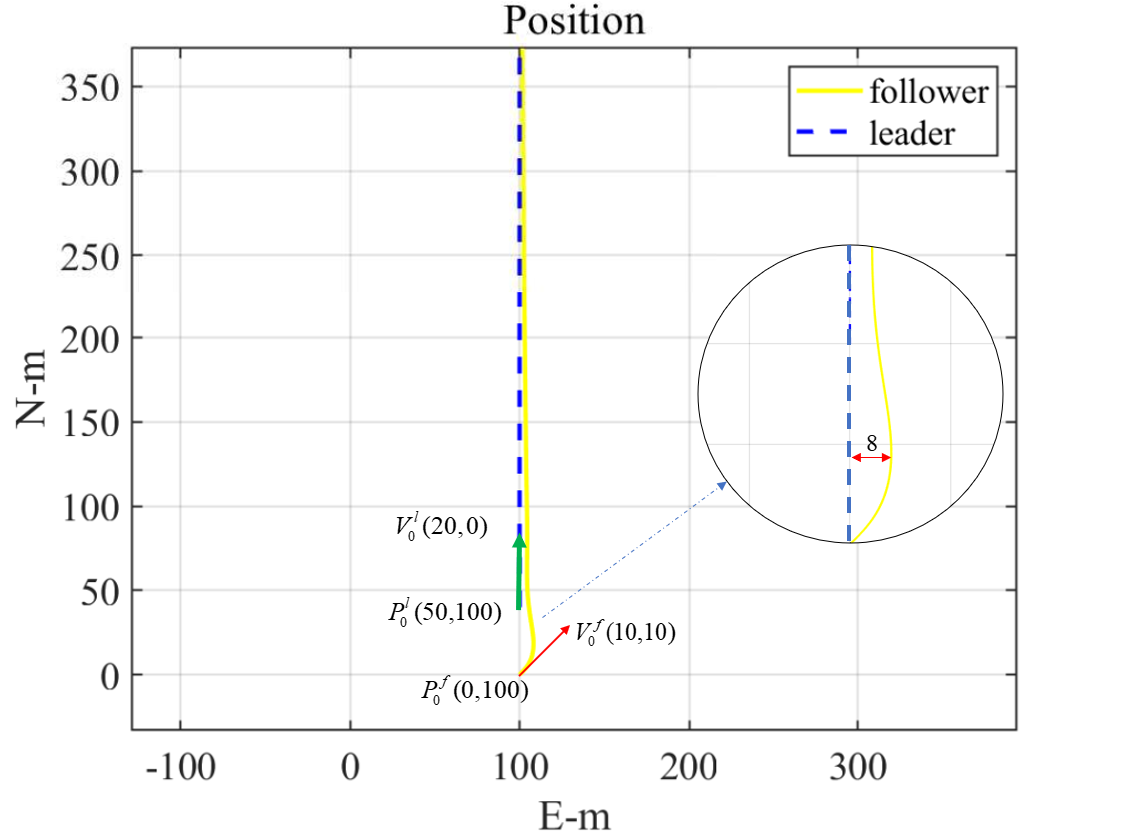
\includegraphics[width=0.85\textwidth]{figures/c5/c5-matlab-pos.png}
    \caption{水平面双机编队位置关系}\label{fig:c5-matlab-pos}
\end{figure}
\begin{figure}[H]
    \centering
    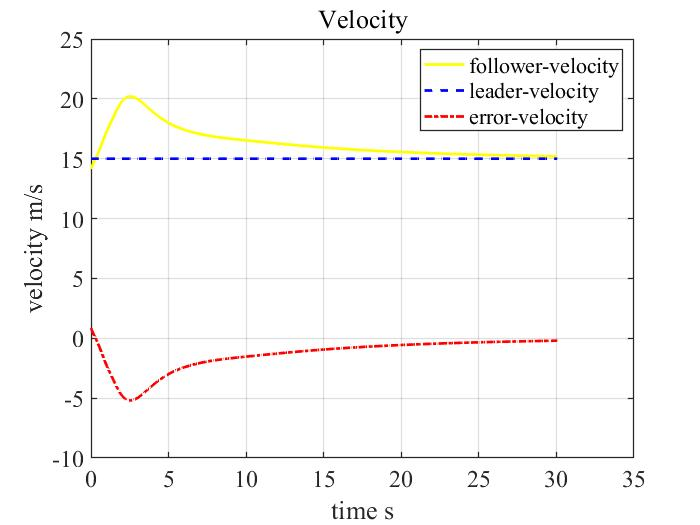
\includegraphics[width=0.85\textwidth]{figures/c5/c5-matlab-vel.jpg}
    \caption{水平面双机速度大小关系}\label{fig:c5-matlab-vel}
\end{figure}
\begin{figure}[H]
    \centering
    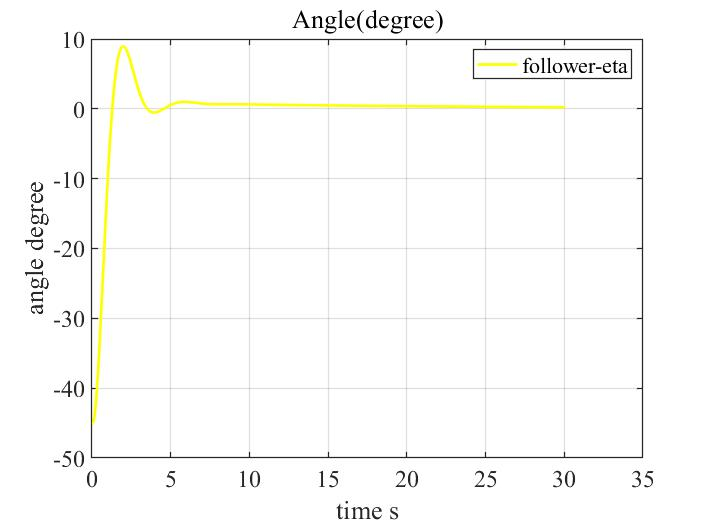
\includegraphics[width=0.85\textwidth]{figures/c5/c5-matlab-eta}
    \caption{水平面双机航迹角关系}\label{fig:c5-matlab-eta}
\end{figure}

竖直平面内,由于控制器的任务是消除高度误差以及追踪来自水平平面控制器的期望速度,控制量将是期望推力$T^{des}$以及期望俯仰角$\theta^{des}$,因而需要引入竖直平面内的无人机动力学模型(参见式\ref{point_dynamaic});按照之前的假设,无人机姿态内环为理想环节,可以用一个时间常数为$\tau_{\theta}$的惯性环节代替之。再结合式\ref{fol_motion_eauation},可以进行竖直平面的相关仿真:
仿真时的领机从机初始运动学量为:
\begin{table}[H]
    \centering
    \caption{竖直面内数学仿真初始运动学量} \label{tab:matlab_vel_cond}
    \begin{tabular*}{0.9\textwidth}{@{\extracolsep{\fill}}c|cc}
        \toprule
        指标 & 初速度(m/s)    & 初始高度(m)\\
        \midrule
        领机 & 20.0  & 10.0\\
        从机 & 10.0 & 100.0\\
        \bottomrule
    \end{tabular*}
\end{table}
竖直内TECS控制器的参数如下表所示:
\begin{table}[H]
    \centering
    \caption{竖直面内TECS控制器参数} \label{tab:matlab_TECS_param}
    \begin{tabular*}{0.9\textwidth}{@{\extracolsep{\fill}}c|cccc}
        \toprule
        TECS参数 & 油门时间常数 & 俯仰角时间常数 & 俯仰角阻尼 & 油门阻尼   \\
        \midrule
        值       & 4.0            & 3.0              & 0.7        & 0.65   \\
        \bottomrule
    \end{tabular*}
\end{table}
\begin{table}[H]
    \centering
    \caption{竖直面内TECS控制器参数(续表)} \label{tab:matlab_TECS_param_app}
    \begin{tabular*}{1.0\textwidth}{@{\extracolsep{\fill}}c|cccc}
        \toprule
        TECS参数 & 积分增益 & 俯仰角-速度比重常数 & 高度误差比例增益 & 速度误差比例增益  \\
        \midrule
        值       & 0.3      & 1.0                   & 0.05             & 0.02     \\
        \bottomrule
    \end{tabular*}
\end{table}

为了方便读图,现在将$NED$坐标系下的$D$轴取反之后并用“$height$”表示,
仿真的结果如下三图所示:
\begin{figure}[H]
    \centering
    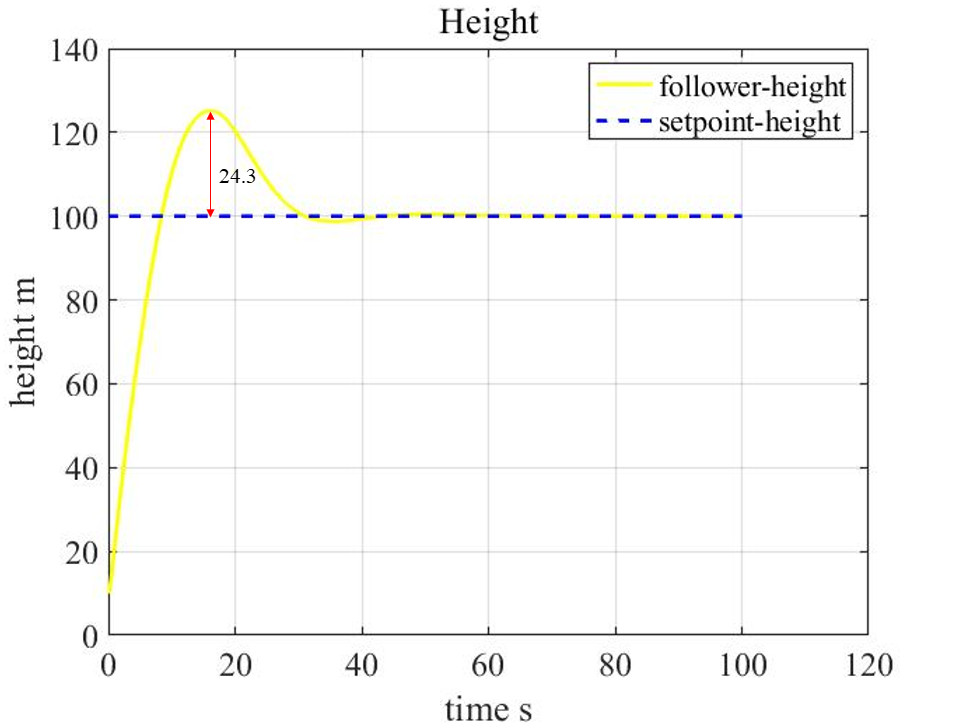
\includegraphics[width=0.85\textwidth]{figures/c5/c5-TECS-height.jpg}
    \caption{竖直平面高度关系}\label{fig:c5-TECS-height}
\end{figure}
\begin{figure}[H]
    \centering
    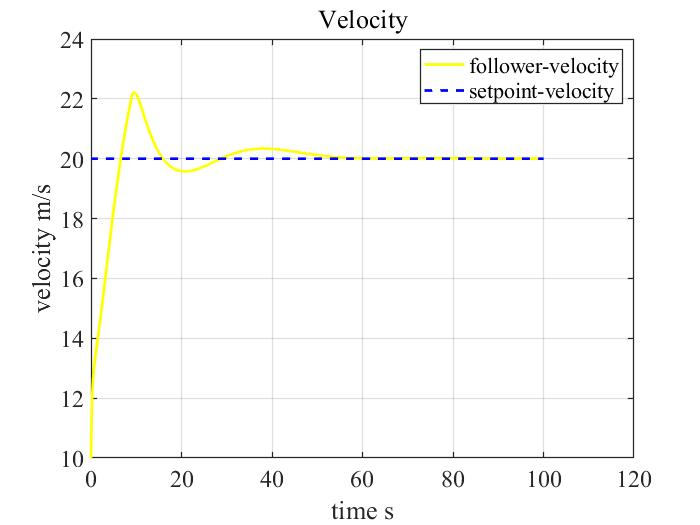
\includegraphics[width=0.85\textwidth]{figures/c5/c5-TECS-vel.jpg}
    \caption{竖直平面速度关系}\label{fig:c5-TECS-vel}
\end{figure}
\begin{figure}[H]
    \centering
    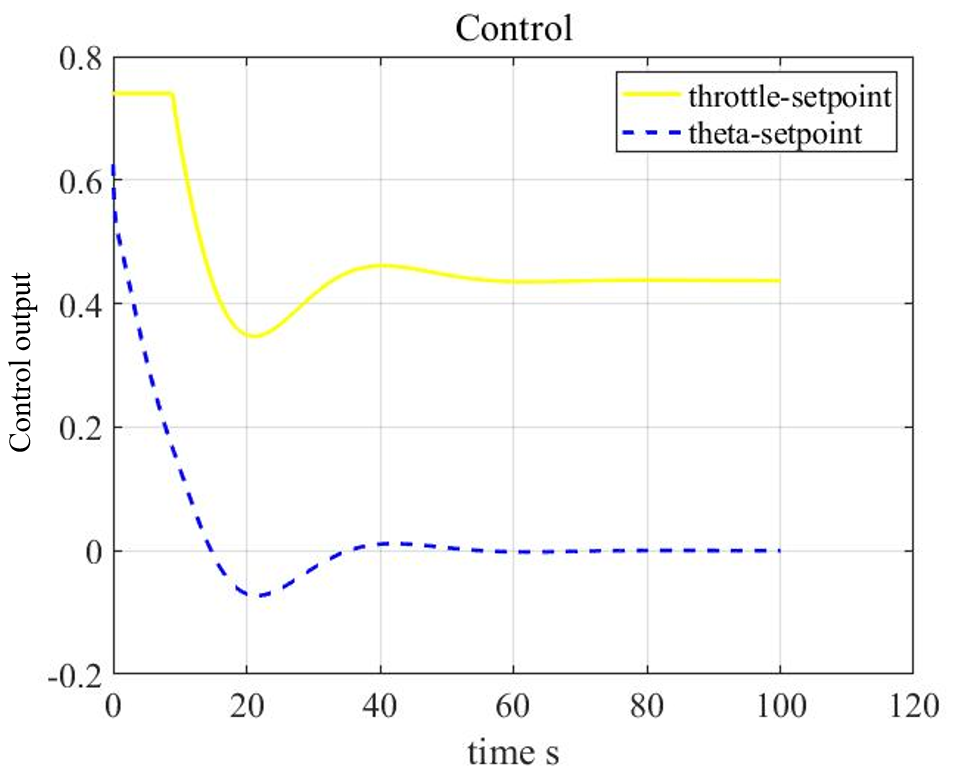
\includegraphics[width=0.80\textwidth]{figures/c5/update/control_output}
    \caption{竖直平面控制量关系}\label{fig:c5-TECS-control}
\end{figure}
由仿真结果可知,本文所设计的TECS控制器可以完成对于期望速度以及期望高度的跟踪,从而达到消除竖直平面内的误差的作用。
\section{基于ROS/Gazebo-PX4的双机编队动力学仿真}
根据第\ref{chap:hardware}章中介绍的ROS-Gazebo仿真环境,进行仿真环境下的双机编队飞行试验。首先利用QGround Control 地面站为领机规划
一条包括起飞以及降落航点在内的一条长直航线。之后先使用地面站将领机1(vehicle 1)
解锁,切换任务模式之后起飞,按照既定航线飞行。等待领机到达第一个
航点之后,再起飞从机2(vehicle 2)
,并切换到外部控制模式,即编队控制的控制逻辑。之后经过一段时间的飞行之后,采集飞行之中的编队误差等数据:最终
编队稳定之后的可视化效果如下:
\begin{figure}[H]
    \centering
    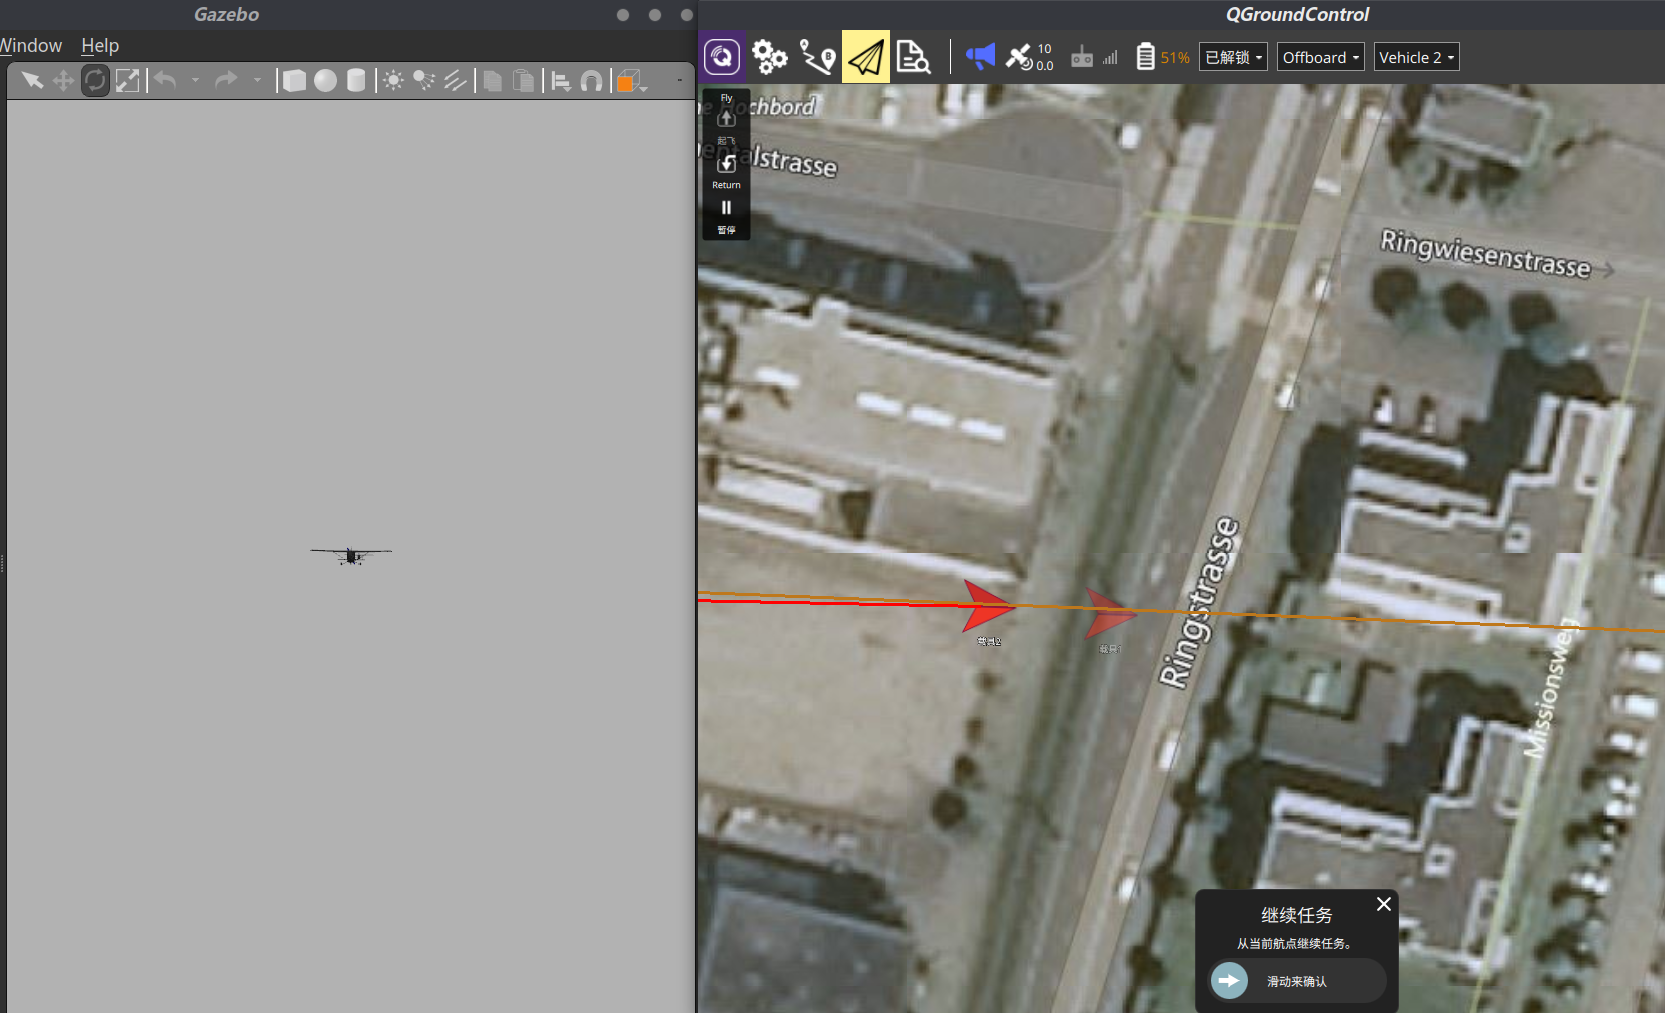
\includegraphics[width=0.85\textwidth]{figures/c5/c5-real-overview}
    \caption{稳定编队之后的编队可视化效果}\label{c5-real-overview}
\end{figure}
动力学仿真的初始条件如下表所示:
\begin{table}[H]
    \centering
    \caption{Gazebo双机编队动力学仿真初始条件} \label{tab:real_init_cond}
    \begin{tabular*}{0.9\textwidth}{@{\extracolsep{\fill}}c|cccc}
        \toprule
        指标     & 初速度(m)     & 初始位置(m)  & 航迹角(°) & 高度(m)  \\
        \midrule
        领机     & (0.0,0.0)    & (0.0,80.0) & 90    & 100.0 \\
        从机     & (0.0,15.0) & (0.0,0.0)   & 90    & 0.0   \\
        \bottomrule
    \end{tabular*}
\end{table}
动力学仿真过程中的编队控制器的控制器参数如下表所示:
\begin{table}[H]
    \centering
    \caption{水平面内控制器参数} \label{tab:real_PID_param}
    \begin{tabular*}{0.9\textwidth}{@{\extracolsep{\fill}}c|ccccc}
        \toprule
        参数 & 比例$K_P$     & 积分$K_I$    & 微分$K_D$ & 混合参数1 & 混合参数2  \\
        \midrule
        X & 0.3 & 0.01  & 0.008  & 0.4   & 0.65 \\
        Y & 0.4 & 0.005 & 0.0015 & 0.005 & 0.4 \\
        \bottomrule
    \end{tabular*}
\end{table}
TECS控制器的参数如下表所示:
\begin{table}[H]
    \centering
    \caption{竖直面内TECS控制器参数} \label{tab:real_TECS_param}
    \begin{tabular*}{0.9\textwidth}{@{\extracolsep{\fill}}c|cccc}
        \toprule
        TECS参数 & 油门时间常数 & 俯仰角时间常数 & 俯仰角阻尼 & 油门阻尼   \\
        \midrule
        值       & 8            & 5              & 0.3        & 0.5   \\
        \bottomrule
    \end{tabular*}
\end{table}
\begin{table}[H]
    \centering
    \caption{竖直面内TECS控制器参数(续表)} \label{tab:real_TECS_param_app}
    \begin{tabular*}{1.0\textwidth}{@{\extracolsep{\fill}}c|cccc}
        \toprule
        TECS参数 & 积分增益 & 俯仰角-速度比重常数 & 高度误差比例增益 & 速度误差比例增益  \\
        \midrule
        值      & 0.1  & 1          & 0.05     & 0.02     \\
        \bottomrule
    \end{tabular*}
\end{table}
在仿真过程中,利用ROS提供的rosbag等数据记录工具,可以进行仿真之中的数据记录与处理:
图\ref{c5-real-pos_err_x}-图\ref{c5-real-pos_err_z}分别代表了双机编队位置误差投影
在从机坐标系$O_kx_ky_kz_k$中的分量随时间的变化关系;图\ref{c5-real-eta_err}代表从
机与领机的速度方向误差随时间变化关系;图\ref{c5-real-vel_err}代表从机与领机的速度大小误差随时间的变化关系。
\begin{figure}[H]
    \centering
    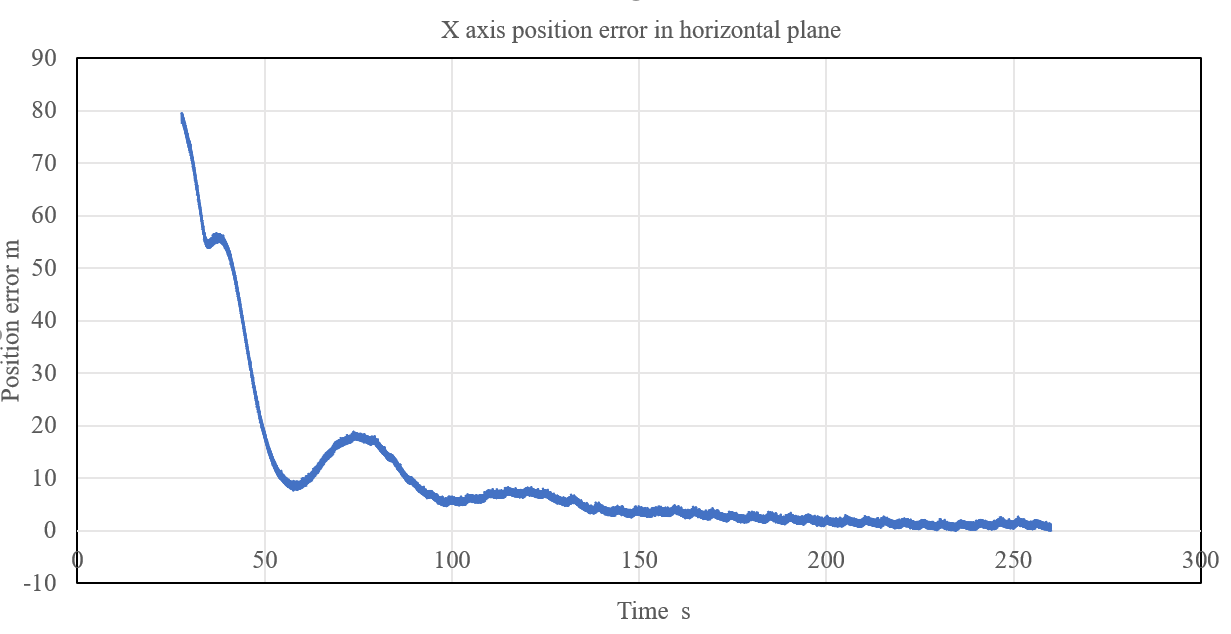
\includegraphics[width=0.85\textwidth]{figures/c5/update/pos_x}
    \caption{X通道位置误差}\label{c5-real-pos_err_x}
\end{figure}
\begin{figure}[H]
    \centering
    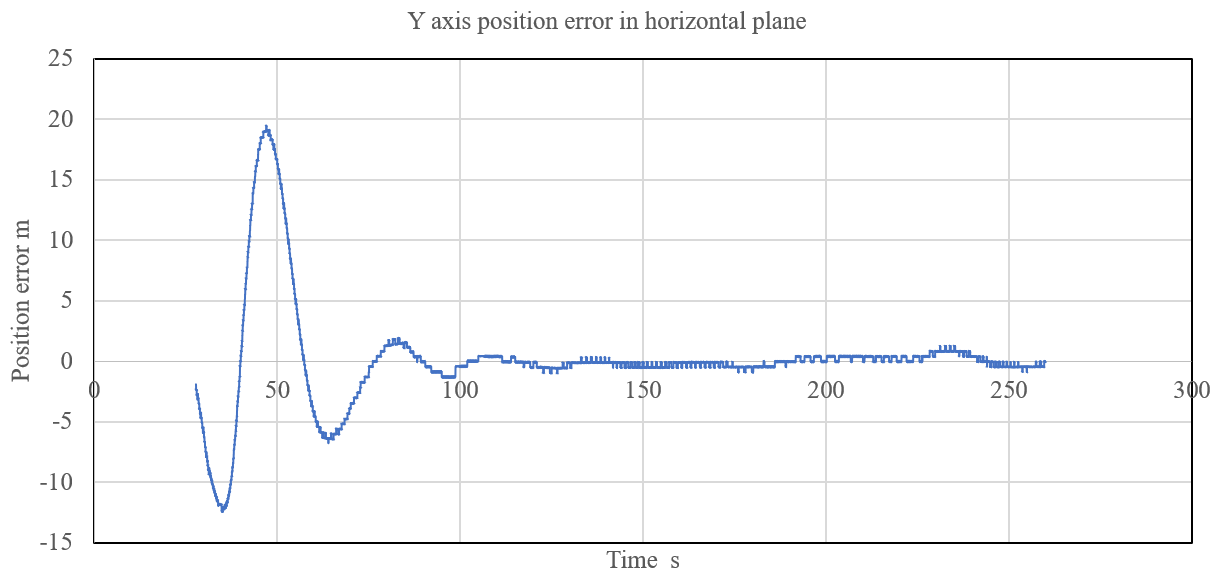
\includegraphics[width=0.85\textwidth]{figures/c5/update/pos_y}
    \caption{Y通道位置误差}\label{c5-real-pos_err_y}
\end{figure}
\begin{figure}[H]
    \centering
    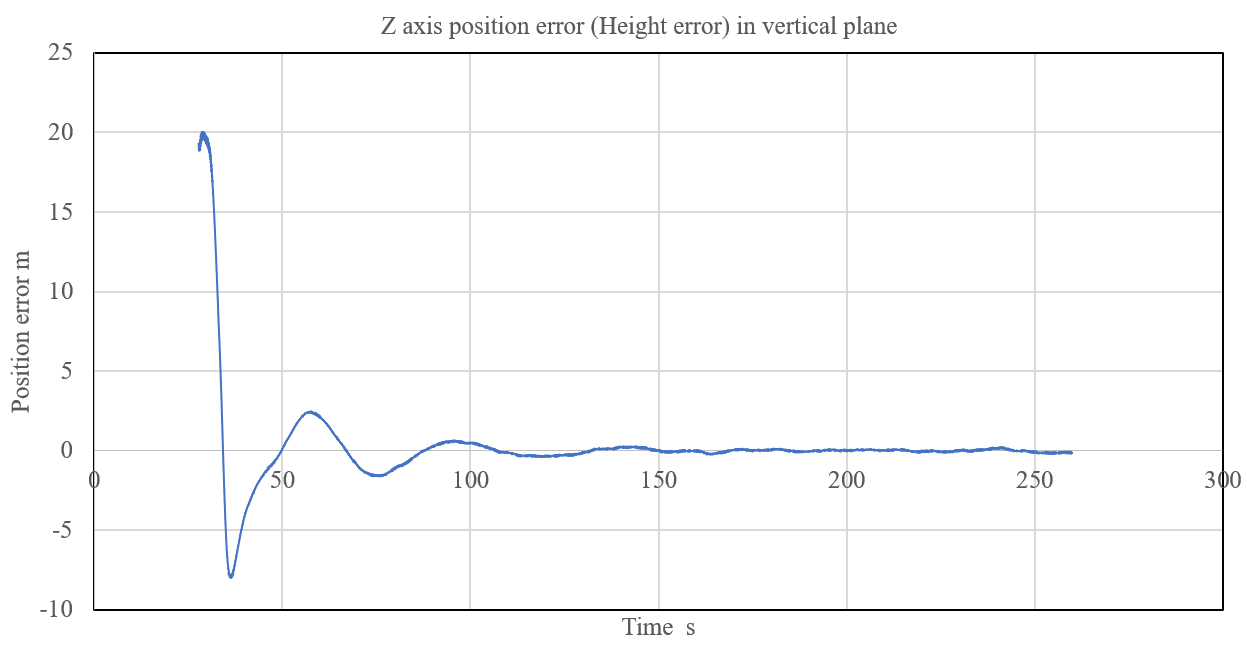
\includegraphics[width=0.85\textwidth]{figures/c5/update/pos_z}
    \caption{Z通道位置误差}\label{c5-real-pos_err_z}
\end{figure}
\begin{figure}[H]
    \centering
    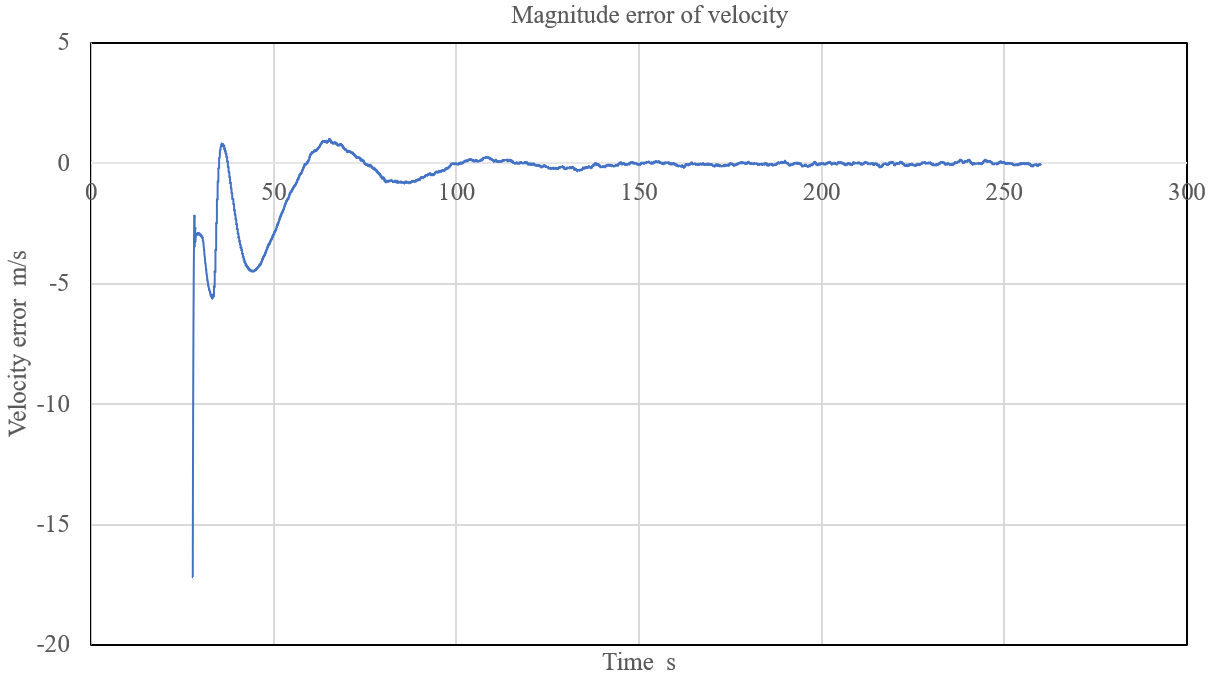
\includegraphics[width=0.85\textwidth]{figures/c5/update/vel}
    \caption{领机从机速度大小误差}\label{c5-real-vel_err}
\end{figure}
\begin{figure}[H]
    \centering
    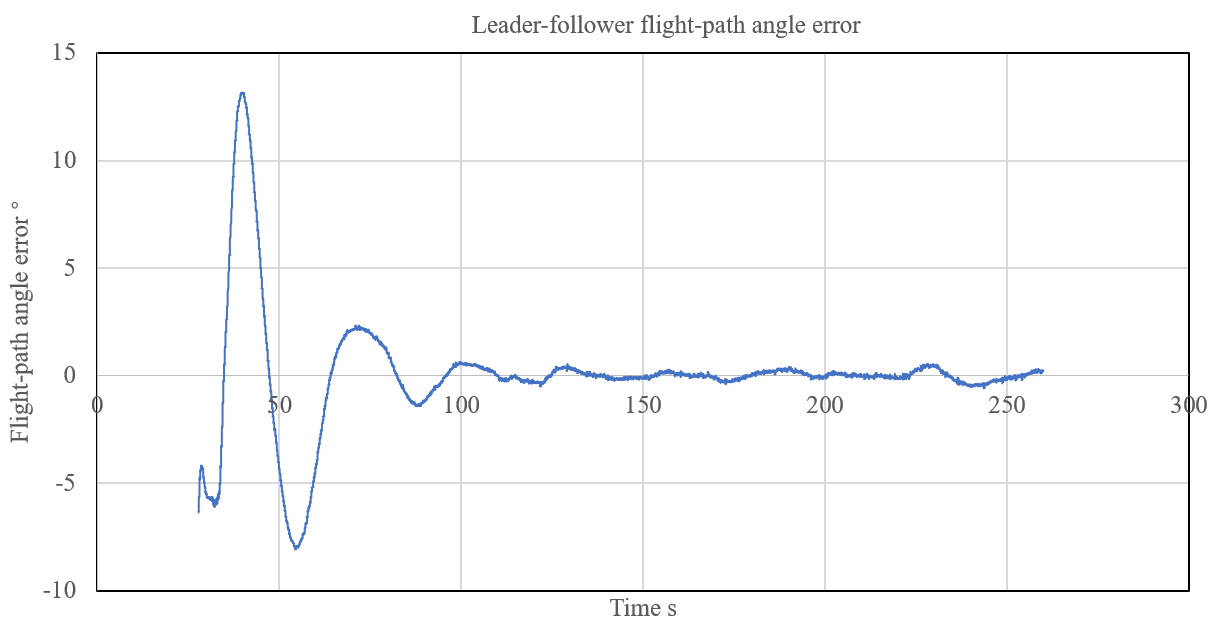
\includegraphics[width=0.85\textwidth]{figures/c5/update/angle}
    \caption{领机从机航迹角误差}\label{c5-real-eta_err}
\end{figure}
需要注意的一点是:此处的位置误差指的是从机的实际位置与编队的期望位置之间的位值误差,而并非与领机的位置误差。
从图\ref{c5-real-pos_err_x}-图\ref{c5-real-pos_err_z}中可看出,编队的3通道位置误差最终稳定在$\pm0.1m$范围之内;而无人机的翼展尺寸在$2m$左右
则按照文献\cite{Zhang2017Aerodynamics},此种精度可以满足固定翼无人机紧密编队的要求。

从动力学仿真的结果来看,速度的收敛速度要迟于位置的收敛,这是因为从机速度要大于领机的速度时才可以消除相应的位置误差。但是最终速度
方向以及速度大小均会收敛到
领机的速度方向以及大小,从而实现前文所提出的无人机编队的位置以及速度要求。需要说明的一点是:在图\ref{c5-real-eta_err}中,速度的
角度误差较长时间收敛到0,是因为无人机的协调转弯的过渡时间较长所导致的:两种转弯模式,侧滑转弯(STT)基于侧滑角产生侧向力,本方式的侧向过载较小;
协调(倾斜)转弯:滚转后使升力对准所需机动方向,获得的侧向过载大,但是过渡时间长。\cite{YuJianQiao2010}上述原因,导致无人机内环在
控制航向时过渡时间较大。

\section{双机编队数学仿真和动力学仿真的关系对比}
本章中所用到的两种仿真方法的侧重点有所不同,所使用的方法也有所不同,
因而导致所出现的仿真结果也不尽相同。

对于数学仿真而言,该仿真方法专注于编队控制器控制逻辑以及控制规律的
可行性验证:其根本目的是检验控制器设计时,选取的混合误差以及所选择
的解耦控制的方法是否可行。

对于动力学仿真而言,该仿真是建立在数学仿真验证通过的基础之上的,其目的:
是检验前文逻辑可行的编队控制器在考虑无人机自驾仪的姿态控制以及无人机
动力学的环节之后的控制稳定性。

在实现仿真的方法上,两种仿真仿真方法的主要区别在于编队控制器的控制
对象的动态特性的不一致:数学仿真的控制对象实际上是一个时间常数为
$\tau$的一阶惯性环节和第\ref{chap:formation_dynamic_equ}中介绍的
无人机质点运动学的结合;而动力学仿真的控制对象是完整的自动驾驶仪内环
以及无人机动力学所组成的更加复杂、控制难度更高的动力学环节,能够比较
真实地反映出编队的状态。下图展示了两种仿真方法的实现方法:
\begin{figure}[H]
    \centering
    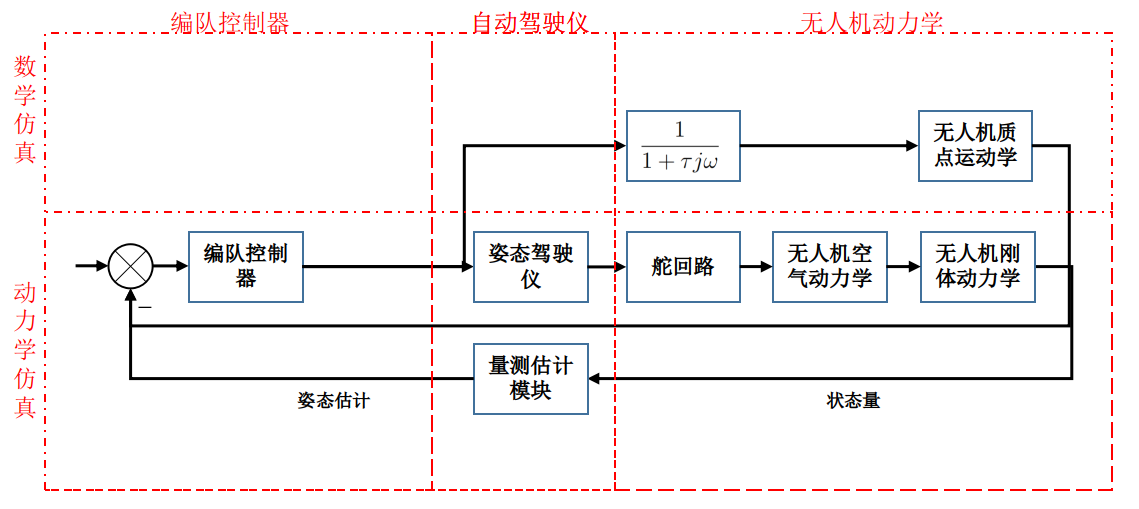
\includegraphics[width=0.85\textwidth]{figures/adds/contrust_sim}
    \caption{数学与动力学仿真实现方法}\label{fig:contrust_sim}
\end{figure}

在仿真结果上,动力学仿真相较于数学仿真,控制收敛时间明显加长,超调
量增大,稳态误差也有一定程度的增加,控制效果整体恶化。除去控制对象
本身的复杂性,动力学仿真环境产生的传感器噪声以及环境不确定性也使得控制
对象的复杂难度增加。
\section{本章小结}
本章主要分为三部分:第一部分着重介绍了本次设计所需要用到的仿真软件环境,详细介绍了Gazebo的软件架构,仿真机理以及仿真的相关特性。并通过ROS操作系统以及
MAVROS功能包搭建了与PX4内环进行数据交互的软件接口;之后结合Gazebo建立起了完整的编队控制器的无人机动力学仿真实验环境,
为后文的动力学仿真提供了相应的平台。
之后的主要工作是对于前文所设计的编队控制器进行响应的仿真:在第二部分,考虑无人机的质点运动模型,利用MATALB/Simulink等工具进行了
编队控制器的算法层面的数学仿真。在第三部分,利用前文中所介绍的Gazebo仿真环境进行编队控制器的动力学仿真,并整定了相关控制器的
参数,检验了控制器的稳定性,最后对两种仿真方式的关系做出了对比。

\chapter{无人机编队整体控制逻辑、仿真环境以及硬件选型}
\label{chap:hardware}
上一章中完整地介绍了编队控制器的设计方法,以及实际应用时的改进;
本章主要介绍无人机编队的编队控制算法之外的系统组成部分;之后介绍无人机编队的整体的控制的实现逻辑,之后将介绍无人机编队的动力学仿真环境的搭建。
最后将介绍本次设计之中所用到的无人机型号,自动驾驶仪硬件以及姿态自动驾驶仪内环基本控制逻辑。
\section{ 软件控制逻辑以及软件环境 }
编队控制算法所运行的软件环境是ROS(Robot Operating System, 机器人操作系统)。ROS是一个为机器人开发而设计的
开源类操作系统平台。本质上,ROS是一个运行于实际操作系统上的应用程序,因而与实际的操作系统有着本质的区别,
但是其对于硬件的抽象以及应用层程序之间的通信的支持使其具有
操作系统的一些重要特征。ROS提供的进程间的通讯方式多种多样,针对于不同要求的应用场景
则设计了不同的进程间的通讯方式,例如消息(Message)、服务(Service)和参数(Param)等;
由于ROS开源社区的蓬勃发展,越来越多的第三方库可以供给开发者使用,也使得针对无人机的
应用开发变得十分方便。本次使用的应用程序接口是
ROS下的mavros功能包,
本功能包的作用是:将来自自动驾驶仪的无人机状态数据由mavlink通信协议转换为ROS的进程间的通讯的协议;
将来自编队控制器的姿态驾驶仪内环的期望姿态角以及期望油门值按照mavlink的协议进行编码,从而起到沟通编队控制器以及姿态驾驶仪内环的桥梁作用。
这里涉及到的Mavlink通讯协议,最早由苏黎世联邦理工大学的研究人员开发,是一种十分轻量级的消息传递协议,广泛用于当今的无人机通讯
,以及无人机内部组件以及无人机与地面站之间的通讯。
MAVLink遵循现代的混合发布-订阅和点对点设计模式:数据流作为主题发送/发布,而配置子协议(如任务协议或参数协议)是点对点重传。
MAVlink通讯已经作为一个专用库封装和发布,通讯时只需要调用相应的库函数进行打包以及包解析,无需再自行定义消息传输格式。
自动驾驶仪则使用第\ref{chap:formation_dynamic_equ}章中介绍的PX4开源自驾仪,此处不再赘述。
\section{无人机软硬件环境选配}
本文所设计的编队控制器是以开源自动驾驶仪PX4的内环为基础的,PX4的内环自动驾驶仪运行在Pixhawk这一开源硬件之上,成为上层控制的下位机(slave computer):
编队控制算法运行在具有ROS环境的上位机(host computer)中;
整体的软件硬件选配关系如下图所示:
\begin{figure}[H]
    \centering
    \includegraphics[width=1\textwidth]{figures/c4/c4-soft-hard.png}
    \caption{硬件软件选配关系}\label{fig:c4-soft-hard.png}
\end{figure}
上位机(host computer)的选择主要由其性能决定,应满足ROS基本环境的正常运行以及编队控制算法的需求;其次应考虑该硬件的寿命,体积,工况
要求等指标。下位机(slave computer)是PX4等算法运行的介质,也是飞行之中的重要传感器如惯性原件(IMU)、磁罗盘以及定位模块(GPS Module)的
工作平台,选择时考虑其传感器精度,平台计算能力等因素;无人机是编队控制的载具平台,应根据上述硬件以及必要航电设备选择翼面积、起飞质量
有效载荷等重要参数;根据硬件安放位置选择合适的机舱外形;根据编队控制需要确定平飞速度;根据期望推力选择发动机型号;根据起飞降落方式
选择起落架类型。必要时,应根据性能要求以及指标设计无人机。

在实现无人机编队过程中,双机通信必不可少。通信模块相对于无人机系统相对独立,在此只介绍硬件实现的一种手段:通讯模块选用P900芯片,通讯协议
选用mavlink协议,驱动由ROS下的串口功能包“serial”提供;领机将自身的状态信息通过串口从其自动驾驶仪滤波之后的值中获取
,之后进行mavlink的编码,最后通过数传模块发送之后,接收端进行解包;实际双机编队飞行试验的硬件链接逻辑如下图所示:
\begin{figure}[H]
    \centering
    \includegraphics[width=1\textwidth]{figures/c4/double_plane_real}
    \caption{双机编队硬件链接}\label{fig:c4-double_plane_real}
\end{figure}
\section{无人机编队动力学仿真环境}
所谓无人机动力学仿真环境,是在考虑无人机的动力学过程的基础之上搭建的仿真环境,相较于控制器的数学仿真,此种仿真环境考
虑了无人机作为一个实际的被控系统而存在的过渡过程,不确定性以及扰动因素,将更加还原无人机飞行时的实际状态。
本次动力学仿真环境基于Gazebo这一通用的开源仿真环境,除调用物理引擎仿真飞行器6自由度的动力学模型外,还可以产生相应的、添加噪声
污染的传感器数据反馈给下位机自动驾驶仪。
\begin{figure}[H]
    \centering
    \includegraphics[width=0.75\textwidth]{figures/c4/Gazebo.png}
    \caption{Gazebo仿真环境}\label{fig:c4-Gazebo}
\end{figure}

Gazebo仿真环境可看做由世界(World)、模型(Model)、传感器(Sensor)、物理引擎(Physical Engine)以及插件(Plugin)等模块
组成:世界(World)包含了仿真所使用的全部组件,例如模型(Model)、传感器(Sensor)、灯光(Light)等;模型(Model)的是构成
构成世界的组成部分,可以多次复用。传感器(Sensor)是一类特殊的模型,可以产生带有噪声的传感器数据信息。物理引擎(Physical Engine)
是驱动模型运动的组件,对应的物理库为基本仿真组件提供了一个简单和通用的界面,包括刚体、碰撞形状和表示关节约束的关节。
这个接口集成了四个开源物理引擎。

Gazebo在仿真时,首先加载世界,包括其中的各种参数如重力场定义、灯光等,以及定义了飞机4通道操纵机构飞机模型;
之后,各类插件,例如空气动力学插件、传感器插件以及环境插件等调用物理引擎接口,产生诸如无人机刚体运动学,传感器噪声
、大气环境等相关等相关仿真过程量。至此,通过Gazebo的GUI可以在可视化界面上得到无人机的运动图像。通过PX4官方给出的仿真工具,
可将在Gazebo中运行的固定翼无人机传感器的测量原始信息编码成MAVlink消息格式,反之亦然,之后,再通过TCP4560端口与PX4自驾仪进行通讯,即
Gazebo中的相应控制舵面运动的插件接受来自PX4的控制器信息,再将仿真的传感器数据进行打包和发送,从而构成了仿真环境。

总而言之,Gazebo考虑了无人机详细的动力学方程,只是在空气动力和力矩的产生方面,使用了简单的工程化的计算方法,使用速度、翼面积、
升阻系数等来计算无人机所受的力和力矩,无法模拟细致入微的空气动力学特性;因而不能使用Gazebo环境进行诸如油耗测试等涉及空气动力学
影响的仿真实验。但是,作为编队控制器设计与仿真阶段,Gazebo不失为一种强大的验证算法的手段。

另外,仿真之中的飞机的动力学模型由Gazebo仿真环境给出,可自定义飞机的质量,推力等参数;仿真之中的传感器数据由Gazebo产生,由PX4读取,作为
真实环境之中的传感器数据的仿真。上述参量均可以按照本次无人机平台做出相应的修改。

基于ROS的编队控制程序同时运行,通过mavros等程序API进行数据交互,完成动力学仿真。
相应的仿真程序之间的逻辑关系如下图所示:
\begin{figure}[H]
    \centering
    \includegraphics[width=0.75\textwidth]{figures/c4/px4_sitl_overview.png}
    \caption{编队控制仿真逻辑}\label{fig:px4_sitl_overview}
\end{figure}
在启动双机仿真时,启动脚本会加载两个无人机模型,并将与其相关的ROS消息用形如“UAV0、UAV1”等编号形式进行区分。
%TODO:需要添加Gazebo的动力学模型是如何载入进来的。
\section{本章小结}
本章着重介绍了本次设计所需要用到的仿真软件环境,详细介绍了Gazebo的软件架构,仿真机理以及仿真的相关特性。并通过ROS操作系统以及
MAVROS功能包搭建了与PX4内环进行数据交互的软件接口;之后结合Gazebo建立起了完整的编队控制器的无人机动力学仿真实验环境,
为后文的动力学仿真提供了相应的平台。


% 结论:在结论相应的 TeX 文件处进行结论部分的撰写
%%
% The BIThesis Template for Bachelor Graduation Thesis
%
% 北京理工大学毕业设计(论文)结论 —— 使用 XeLaTeX 编译
%
% Copyright 2020 Spencer Woo
%
% This work may be distributed and/or modified under the
% conditions of the LaTeX Project Public License, either version 1.3
% of this license or (at your option) any later version.
% The latest version of this license is in
%   http://www.latex-project.org/lppl.txt
% and version 1.3 or later is part of all distributions of LaTeX
% version 2005/12/01 or later.
%
% This work has the LPPL maintenance status `maintained'.
%
% The Current Maintainer of this work is Spencer Woo.
%
% Compile with: xelatex -> biber -> xelatex -> xelatex

\chapter*{\vskip 10bp\textmd{结~~~~论} \vskip -6bp}
\addcontentsline{toc}{chapter}{结~~~~论}

% 在结论部分的子标题不需要序号,加上 * 即可(一个例子如下)
% \section*{结论段落标题}

% 这里插入一个参考文献,仅作参考
本文以固定翼无人机的紧密编队为研究对象,设计了一种符合现有开源无人机自动驾驶仪(PX4)姿态环输入的编队控制器。并利用MATLAB/Simulink对
无人机编队算法进行了运动学层面上的仿真验证;最后,使用ROS-Gazebo动力学仿真环境,对文中所设计的编队控制器进行了动力学层面上的
仿真。上述两种仿真的结果均显示此种控制器可以完成固定翼的紧密编队控制。

本文的主要研究结果如下:
\begin{enumerate}
    \item 明确了编队控制器设计需要使用的飞行力学以及导航坐标系,并在相应坐标系中将无人机的三维空间运动进行了简化,分为竖直以及水平
        两个通道分别控制;之后,按照简化的无人机运动,定义描述无人机编队的物理量;最后,建立了单架无人机运动学方程组。
    \item 以当下开源自动驾驶仪PX4为基础,介绍单架无人机的控制逻辑实现:包括导航模块、位置控制模块以及姿态控制模块的控制逻辑;最后介绍
        PX4的整理软件架构。
    \item 对于编队控制器进行设计:首先定义了编队误差的基本形式,根据控制的需要找出对应的控制输入。再利用增量式PID对于编队控制器进行控制;
        得到编队控制器的数学形式,将第一步完成的编队控制器期望值设计总能量控制器(TECS)进行再次转化,最终得到内环控制器对应的编队控制
        器的完整形式,编队控制器的输入为编队的位置误差,速度大小以及速度方向误差所定义的混合误差,控制器的输入是与姿态驾驶仪内环对应的
        无人机期望姿态以及期望推力。
    \item 对文中所得到的编队控制器利用MATLAB等工具进行数学仿真:利用文中提出的无人机编队的质点运动模型,不考虑无人机的姿态动力学过程,仅
        验证编队控制的控制逻辑的正确性。得到了相关的仿真实验数据以及结果图。
    \item 将文中提出的编队控制器利用C/C++编程语言,结合ROS操作系统的要求,进行向硬件平台的移植,并进行工程实际应用时的优化。在考虑无人机的姿态动力学、运动学
        传感器噪声以及大气环境不确定性等因素的条件下,对于所提出的编队控制器进行动力学仿真。在此过程中,结合现有的PX4-QGroundControl地面站以及ROS
        所提供的rosbag等工具对编队过程进行记录和监视,经过参数调节以及优化,最终得到编队控制器在动力学仿真环境下的应用效果。
\end{enumerate}
本文中所设计控制器还有很大的改进空间:首先,由于固定翼无人机速度的动力学惯性很大,尤其在速度大于期望速度的情况下,飞机减速的响应速度不佳,
在后续的设计改进之中应考虑固定翼无人机速度控制的特殊之处。其次,横侧向控制器中控制速度方向的部分优先级应该高于其他,但为了调整和参数
的方便性,因而将横侧向角度和位置误差进行混合。

文中仅仅设计以及仿真验证了一种基于现有开源自动驾驶仪的编队控制器,
项目后续工作,应按照前文所设计的编队控制实验的相关方法进行下一步的
实物实验工作。

% 参考文献:如无特殊需要,参考文献相应的 TeX 文件无需改动,添加参考文献请使用 BibTeX 的格式
%   添加至 misc/ref.bib 中,并在正文的相应位置使用 \cite{xxx} 的格式引用参考文献
\input{misc/4_reference.tex}
% 附录:在附录相应的 TeX 文件处进行附录部分的撰写
%\input{misc/5_appendix.tex}
% 致谢:在致谢相应的 TeX 文件处进行致谢部分的撰写
\input{misc/6_acknowledgements.tex}

\end{document}
